

%!TEX root = IntroArithGrps.tex

\mychapter{\texorpdfstring{Arithmetic Subgroups\\of Classical Groups}%
	{Arithmetic Subgroups of Classical Groups}}
\label{ArithClassicalChap}

\prereqs{Restriction of Scalars (\cref{RestrictScalarsSect}) and examples of arithmetic subgroups (\cref{EgArithGrpsChap}).}


This \lcnamecref{ArithClassicalChap} will give a quite explicit description (up to commensurability) of all the arithmetic subgroups of almost every classical Lie group~$G$ \csee{ArithLattsAreClassical}. (Recall that a simple Lie group~$G$ is ``classical'' if it is either a special linear group, an orthogonal group, a unitary group, or a symplectic group \csee{ClassicalDefn}.) The key point is that all the $\rational$-forms of~$G$ are also classical, not exceptional, so they are fairly easy to understand. 
However, there is an exception to this rule: some $8$-dimensional orthogonal groups have $\rational$-forms of so-called ``\index{triality}triality type'' that are not classical and will not be discussed in any detail here \csee{D4weird}.
%From the correspondence between $\rational$-forms and arithmetic subgroups, this can be thought of as a list of all the arithmetic subgroups of~$G$ (up to commensurability).

Given~$G$, which is a Lie group over~$\real$, we would like to know all of its $\rational$-forms (because, by definition, arithmetic groups are made from $\rational$-forms). However, we will start with the somewhat simpler problem that replaces the fields $\rational$ and~$\real$ with the fields $\real$ and~$\complex$: finding the $\real$-forms of the classical Lie groups over~$\complex$.



\section{\texorpdfstring{$\real$}{R}-forms of classical simple groups over%
\texorpdfstring{~$\complex$}{ C}} \label{RFormsOfCGrps}

To set the stage, let us recall the classical result that almost all complex simple groups are classical:

\begin{thm}[(Cartan, Killing)] \label{AlmostAllOverC}
All but finitely many of the simple Lie groups over\/~$\complex$ are isogenous to either\/ $\SL(n,\complex)$, $\SO(n,\complex)$, or\/ $\Sp(2n,\complex)$, for some~$n$.
\end{thm}

\begin{rem} \label{EFGOverCRem}
Up to isogeny, there are exactly five simple Lie groups over~$\complex$ that are not classical. They are the ``\index{exceptional Lie group}exceptional'' simple groups, and are called $E_6$, $E_7$, $E_8$, $F_4$, and~$G_2$.
%Although we do not need this terminology, each simple group has a \defit[type (of a simple Lie group)]{type}:
%	\begin{itemize}
%	\item $\SL(n,\complex)$ is of type~$A$, 
%	\item $\SO(n,\complex)$ is of type~$B$ or~$D$, depending on whether $n$ is odd or even, respectively,
%	and
%	\item $\Sp(2n,\complex)$ is of type~$C$.
%	\end{itemize}
%The remaining simple groups over~$\complex$ are of type~$E$, $F$, or~$G$. Up to isogeny, there are exactly three of type~$E$, one of type~$F$, and one of type~$G$.
\end{rem}

Now, we would like to describe the $\real$-forms of each of the classical groups. For example, finding all the $\real$-forms of $\SL(n,\complex)$ would mean making a list of the (simple) Lie groups~$G$, such that the ``complexification'' of~$G$ is $\SL(n,\complex)$. This is not difficult, but we should perhaps begin by explaining more clearly what it means.

It has already been mentioned that, intuitively, the complexification of~$G$ is the
complex Lie group that is obtained from~$G$ by replacing
real numbers with complex numbers. 
 For example,
the complexification of $\SL(n,\real)$ is $\SL(n,\complex)$. In general, $G$ is
(isogenous to) the set of real solutions of a certain set of
equations, and we let $G_{\complex}$ be the set of
complex solutions of the same set of equations:

\begin{notation} \label{GxCNot}
 Assume $G \subseteq \SL(\ell,\real)$, for some~$\ell$. Since $G$ is almost Zariski closed \csee{GisAlgic}, there
is a certain subset~$\mathcal{Q}$ of $\real[x_{1,1}, \ldots,
x_{\ell,\ell}]$, such that $G^\circ = \Var(\mathcal{Q})^\circ$. Let
 $$ G_{\complex} = \Var_{\complex}(\mathcal{Q})
 = \{\, g \in \SL(\ell,\complex) \mid \mbox{$Q(g) = 0$, for
all $Q \in \mathcal{Q}$} \,\} .$$
 Then $G_{\complex}$ is a (complex, semisimple) Lie
group.
 \end{notation}

\begin{eg} \label{GxCEg}
 \ 
 \begin{enumerate}
 \item \label{GxCEg-SL}
 $\SL(n,\real)_{\complex} = \SL(n,\complex)$. 
 \item \label{GxCEg-SO}
 $\SO(n)_{\complex} = \SO(n,\complex)$.
 \item \label{GxCEg-SOpq}
 $\SO(m,n)_{\complex} \iso \SO(m+n,\complex)$
\csee{SOpqxC}.
 \end{enumerate}
 \end{eg}

\begin{defn}
 If $G_{\complex}$ is isomorphic to~$H$, then we say
that 
 \begin{itemize}
 \item $H$ is the \defit{complexification} of~$G$, and that
 \item $G$ is an \defit[R-@$\real$-!form]{$\real$-form} of~$H$.
 \end{itemize}
 \end{defn}

The following result lists the complexification of each classical group.
It is not difficult to
memorize the correspondence. For example, it is obvious
from the notation that the complexification of $\Sp(m,n)$ should be
symplectic. Indeed, the only case that really requires
memorization is the complexification of $\SU(m,n)$
\fullcsee{GxC=}{SUmn}.

\begin{prop} \label{GxC=}
 Here is the complexification of each classical Lie group.
 \noprelistbreak
	 \begin{enumerate} \renewcommand{\theenumi}{\Alph{enumi}}
			\renewcommand{\theenumii}{\roman{enumii}}
	 \item \label{GxC=-SL}
	 Real forms of special linear groups:
	 \noprelistbreak
	 	\begin{enumerate} 
		 \item $\SL(n,\real)_{\complex} = \SL(n,\complex)$,
		 \item $\SL(n,\complex)_{\complex} \iso \SL(n,\complex)
		\times \SL(n,\complex)$,
		 \item $\SL(n,\quaternion)_{\complex} \iso
		\SL(2n,\complex)$,
		 \item \label{GxC=-SUmn}
		 $\SU(m,n)_{\complex} \iso \SL(m+n,\complex)$.
		 \end{enumerate}

	 \item Real forms of orthogonal groups:
	 \noprelistbreak
	 	\begin{enumerate}
		 \item $\SO(m,n)_{\complex} \iso \SO(m+n,\complex)$,
		 \item $\SO(n,\complex)_{\complex} \iso \SO(n,\complex)
		\times \SO(n,\complex)$,
		 \item $\SO(n,\quaternion)_{\complex} \iso
		\SO(2n,\complex)$.
		 \end{enumerate}

	 \item Real forms of symplectic groups:
	 \noprelistbreak
	 	\begin{enumerate}
		 \item $\Sp(n,\real)_{\complex} = \Sp(n,\complex)$,
		 \item $\Sp(n,\complex)_{\complex} \iso \Sp(n,\complex)
		\times \Sp(n,\complex)$,
		 \item $\Sp(m,n)_{\complex} \iso
		\Sp \bigl( 2(m+n),\complex \bigr)$.
		 \end{enumerate}
	 \end{enumerate}
 \end{prop}

Some parts of this \lcnamecref{GxC=} are more-or-less obvious (such as $\SL(n,\real)_{\complex} = \SL(n,\complex)$). A few
other examples appear in \cref{CalcGxCSect} below, and the
methods used there can be applied to all of the cases. In
fact, all of the calculations are straightforward
adaptations of the examples, except perhaps the determination of $\SO(n,\quaternion)_{\complex}$ \csee{SOnHxC}.

Nothing in \cref{GxC=} is very surprising. What is not at all obvious is that this list of real forms is complete:

\begin{thm}[(\'E.\,Cartan)] \label{RformsComplete}
Every real form of\/ $\SL(n,\complex)$, $\SO(n,\complex)$, or\/ $\Sp(n,\complex)$ appears in \cref{GxC=}\/ \textup(up to isogeny\/\textup).
\end{thm}

We will discuss a proof of this \lcnamecref{RformsComplete} in \cref{GaloisCohoRealFormsSect}.


\begin{rems} \label{GxC=tensorprod} \ 
\noprelistbreak
 \begin{enumerate}
 
 \item From \cref{GxC=}, we see that a single complex
group may have several different real forms. However, there are always only finitely many (even for exceptional groups).

 \item \label{GxC=tensorprod-LieAlg}
 The Lie algebra of $G_{\complex}$ is the tensor
product $\Lie G \otimes \complex$ \csee{Lie(GxC)}. This is
independent of the embedding of~$G$ in $\SL(\ell,\complex)$,
so, up to isogeny, $G_{\complex}$ is
independent of the embedding of~$G$ in $\SL(\ell,\complex)$.
%Thus, we will often speak of the complexification of~$G$,
%even if $G$~is not a group of matrices, with the
%understanding that the complexification is not entirely well
%defined \see{GCnotWellDefd}.

 \item \label{GxC=tensorprod-Q}
 We ignored a technical issue in \cref{GxCNot}:
there may be many different choices of~$\mathcal{Q}$ (having
the same set of real solutions), and it may be the case that
different choices yield different sets of complex
solutions. (In fact, a bad choice of~$\mathcal{Q}$ can yield
a set of complex solutions that is not a group.) To
eliminate this problem, we should insist that $\mathcal{Q}$
be maximal; that is,
 $$ \mathcal{Q} = \{\, Q \in \real[x_{1,1}, \ldots,
x_{\ell,\ell}] \mid \mbox{$Q(g) = 0$, for all $g \in G$}
\,\} .$$
 Then $G_{\complex}$ is the Zariski closure of~$G$
(over the field~$\complex$), from which it follows that $G_\complex$, like~$G$, is a semisimple Lie group.
 \end{enumerate}
 \end{rems}

\begin{eg} \label{GCnotWellDefd}
 Because the center of $\SL(3,\real)$ is trivial, we see
that $\SL(3,\real)$ is the same Lie group as $\PSL(3,\real)$.
On the other hand, we have
 $$ \SL(3,\real)_{\complex} = \SL(3,\complex) \not\iso
\PSL(3,\complex) = \PSL(3,\real)_{\complex} .$$
 This is a concrete illustration of the fact that different
embeddings of $G$ can yield different complexifications.
Note, however, that $\SL(3,\complex)$ is isogenous to
$\PSL(3,\complex)$, so the difference between the
complexifications is negligible
\fullccf{GxC=tensorprod}{LieAlg}.
 \end{eg}
 

\begin{exercises}

\item \label{SOpqxC}
 Show that $\SO(m,n)_{\complex} \iso
\SO(m+n,\complex)$. 
 \hint{$\SO(m,n)_{\complex}$ is conjugate to
$\SO(m+n,\complex)$ in $\SL(m+n,\complex)$, because $-1$~is a
square in~$\complex$.}

\item \label{Lie(GxC)}
 Show that the Lie algebra of $G_{\complex}$ is $\Lie G \otimes \complex$.

\end{exercises}







\section{Calculating the complexification of%
	\texorpdfstring{~$G$}{ G}}
\label{CalcGxCSect}

This section justifies \cref{GxC=}, by calculating the complexification of each classical group.

Let us start with $\SL(n,\complex)$. This is already a complex Lie group, but
we can think of it as a real Lie group of twice the
dimension. As such, it has a complexification:

\begin{prop} \label{SLnCxC}
 $\SL(n,\complex)_{\complex} \iso \SL(n,\complex)
\times \SL(n,\complex)$.
 \end{prop}

\begin{proof}
 We should embed $\SL(n,\complex)$ as a subgroup of
$\SL(2n,\real)$, find the corresponding set~$\mathcal{Q}$ of
defining polynomials, and determine the complex solutions.
However, it is more convenient to sidestep some of these
calculations by using restriction of scalars, the method
described in \S\ref{RestrictScalarsSect}.

Define $\Delta \colon \complex \to \complex \oplus \complex$
by $\Delta(z) = (z, \cjg{z})$. Then the vectors $\Delta(1) =
(1,1)$ and $\Delta(i) = (i,-i)$ are linearly independent
(over~$\complex$), so they form a basis of $\complex \oplus
\complex$. Thus, $\Delta(\complex)$ is the $\real$-span
of a basis, so it is a $\real$-form of $\complex \oplus
\complex$. Therefore, letting $V = \complex^{2n}$, we see
that
 $$ V_{\real} = \Delta(\complex^n)
 = \bigl\{\, ( v, \overline{v} )
 \mid v \in \complex^n \, \bigr\} $$
 is a real form of~$V$. Let
 $$ \bigl( \SL(n,\complex) \times 
\SL(n,\complex) \bigr)_{\real}
 = \bigset{
 g \in \SL(n,\complex) \times \SL(n,\complex)
 }{
 g (V_{\real}) = V_{\real}
 } .$$
 Then we have an isomorphism 
 $$\tilde \Delta \colon
\SL(n,\complex) \towith{\iso} \bigl(
\SL(n,\complex) \times \SL(n,\complex) \bigr)_{\real} ,$$
 defined by $\tilde
\Delta(g) = (g,\cjg{g})$, so
 \begin{align*}
  \SL(n,\complex)_{\complex}
 \iso \bigl( [\SL(n,\complex) \times \SL(n,\complex)]_{\real}
\bigr)_{\complex}
 = \SL(n,\complex) \times \SL(n,\complex) 
 . & \qedhere \end{align*}
 \end{proof}

\begin{rems} \ \label{GxC=GxGiff}
 \noprelistbreak
 \begin{enumerate}
 \item Generalizing \cref{SLnCxC}, one can show that if
$G$~is isogenous to a complex Lie group, then $G_\complex$ is isogenous to $G \times G$. 
%For example,
% $$ \SO(1,3)_{\complex}
% \iso \SO(4,\complex)
% \sim \SL(2,\complex) \times \SL(2,\complex)
% \sim \SO(1,3) \times \SO(1,3) $$
% (see \pref{isogTypes-D2-SO4C} and~\pref{isogTypes-D2-SO13}
%of \cref{isogTypes}).
 \item From \cref{SLnCxC}, we see that $G_\complex$ need not be simple, even if $G$~is simple.
However, this only happens when $G$~is complex: if $G$~is
simple, and $G$~is not isogenous to a complex Lie group,
then $G_{\complex}$ is simple.
 \end{enumerate}
 \end{rems}

Although not stated explicitly there, the proof of
\cref{SLnCxC} is based on the fact that $\complex
\otimes_{\real} \complex \iso \complex \oplus \complex$.
Namely, the map
 $$ \mbox{$\complex \otimes_{\real} \complex \to \complex
\oplus \complex$
 defined by $v \otimes \lambda \mapsto \Delta(v) \, \lambda$} $$
 is an isomorphism of $\complex$-algebras. Analogously, understanding the complexification of a group defined from the algebra~$\quaternion$ of quaternions will be
based on a calculation of $\quaternion \otimes_{\real}
\complex$.

\begin{lem} \label{HxC}
 The tensor product $\quaternion \otimes_{\real}
\complex$ is isomorphic to $\Mat_{2 \times 2}(\complex)$.
 \end{lem}

\begin{proof}
  Define an $\real$-linear map $\phi \colon \quaternion \to
\Mat_{2 \times 2}(\complex)$ by
 $$ \phi(1) = \Id, 
 \quad \phi(i)
 = \begin{bmatrix}
 i & 0 \\
 0 & -i
 \end{bmatrix}
 ,
 \quad \phi(j)
 = \begin{bmatrix}
 0 & 1 \\
 -1 & 0
 \end{bmatrix}
 ,
 \quad \phi(k)
 = \begin{bmatrix}
 0 & i \\
 i & 0
 \end{bmatrix}
 .
 $$
 It is straightforward to verify that $\phi$ is an injective
ring homomorphism. Furthermore, $\phi \bigl( \{1,i,j,k\}
\bigr)$ is a $\complex$-basis of $\Mat_{2 \times
2}(\complex)$. Therefore, the map $\hat\phi \colon
\quaternion \otimes \complex \to \Mat_{2 \times
2}(\complex)$ defined by $\hat{\phi}(v \otimes \lambda) = \phi(v)
\, \lambda$ is a ring isomorphism \csee{HxCExer}.
 \end{proof}

\begin{prop} \label{SLnHxC}
 $\SL(n,\quaternion)_{\complex} \iso \SL(2n,\complex)$.
 \end{prop}

\begin{proof}
 From \cref{HxC}, we have
 $$ \SL(n,\quaternion)_{\complex}
 \iso \SL \bigl( n, \Mat_{2 \times 2}(\complex) \bigr)
 \iso \SL(2n,\complex) $$
 \csee{SLnHxCExer,Matd(Matn)}.
 \end{proof}

As additional examples, let us look at the
complexifications of the classical simple Lie
groups that are compact, namely, $\SO(n)$, $\SU(n)$, and $\Sp(n)$. 
As observed in \fullcref{GxCEg}{SO}, we
have $\SO(n)_{\complex} = \SO(n,\complex)$. The other
cases are not as obvious.

\begin{prop} \label{SUnxC}
 $\SU(n)_{\complex} = \SL(n,\complex)$.
 \end{prop}

\begin{proof}
 Let 
 \begin{itemize}
 \item $\sigma \colon \complex \to \complex$,
 \item $\vector{\sigma} \colon \complex^n \to \complex^n$,
and
 \item $\widetilde{\sigma} \colon \SL(n,\complex) \to
\SL(n,\complex)$
 \end{itemize}
 be the
usual complex conjugations $\sigma(z) = \cjg{z}$,
$\vector{\sigma}(v) = \cjg{v}$, and
$\widetilde{\sigma}(g) = \cjg{g}$. We have
 \begin{align*}
 \SU(n) &= \{\, g \in \SL(n,\complex) \mid g^* g = \Id \,\}
\\
 &= \{\, g \in \SL(n,\complex) \mid \widetilde{\sigma}(g^\transpose)
g = \Id \,\} ,
 \end{align*}
 so, in order to calculate $\SU(n)_{\complex}$, we
should determine the map $\widetilde{\eta}$ on $\SL(n,\complex)
\times \SL(n,\complex)$ that corresponds
to~$\widetilde{\sigma}$ when we identify $\complex^n$ with
$(\complex^n \oplus \complex^n)_{\real}$ under the
map~$\vector{\Delta}$. 

First, let us determine $\vector{\eta}$. That
is, we wish to identify $\complex^n$ with~$\real^{2n}$, and
extend $\vector{\sigma}$ to a $\complex$-linear map
on~$\complex^{2n}$. However, as usual, we use the
$\real$-form $\vector{\Delta}(\complex^n)$, in place of
$\real^{2n}$. It is obvious that if we 
	$$ \text{define $\vector{\eta}
\colon \complex^n \oplus \complex^n \to \complex^n \oplus
\complex^n$ by $\vector{\eta}(x,y) = (y,x)$,} $$
then
$\vector{\eta}$ is $\complex$-linear, and the following
diagram commutes:
 $$ 
 \begin{matrix}
 \complex^n & \towith{\vector{\Delta}} & \complex^n
\oplus \complex^n \\
 \mapdown{\vector{\sigma}} & & \mapdown{\vector{\eta}} \\
 \complex^n & \towith{\vector{\Delta}} & \complex^n \oplus
\complex^n 
 . \end{matrix}
 $$
 Thus, it is fairly clear that $\widetilde{\eta}(g,h) = (h,g)$. 
 Hence
 \begin{align*}
 \SU(n)_{\complex}
 &= \{\, (g,h) \in \SL(n,\complex)
\times \SL(n,\complex) \mid \widetilde{\eta} \bigl( g^\transpose,
h^\transpose \bigr) (g,h) = (\Id,\Id) \,\} \\
 &= \{\, (g,h) \in \SL(n,\complex)
\times \SL(n,\complex) \mid \bigl( h^\transpose,
g^\transpose \bigr) (g,h) = (\Id,\Id) \,\} \\
 &= \{\, \bigl( g,(g^\transpose)^{-1} \bigr) 
\mid g  \in
\SL(n,\complex) \,\} \\
 &\iso \SL(n,\complex) .
&& \qedhere \end{align*}
 \end{proof}

\begin{prop} \label{SpnxC}
 $\Sp(n)_{\complex} = \Sp(2n,\complex)$.
 \end{prop}

\begin{proof}
 Let 
 \begin{itemize}
 \item $\phi \colon \quaternion \hookrightarrow \Mat_{2
\times 2}(\complex)$ be the embedding that is described in the proof
of \cref{HxC},
 \item $\tau$ be the usual conjugation on~$\quaternion$, 
 \item $J = 
 \begin{bmatrix}
 0 & 1 \\
 -1 & 0 
 \end{bmatrix}
 $, and
 \item $\eta \colon \Mat_{2 \times 2}(\complex)  \to \Mat_{2
\times 2}(\complex)$ be defined by 
 $\eta(x) = J^{-1} x^{\transpose} J$.
 \end{itemize}
 Then $\eta$ is $\complex$-linear, and the following diagram
commutes:
 $$ 
 \begin{matrix}
 \quaternion & \towith{\phi} & \Mat_{2 \times 2}(\complex) \\
 \mapdown{\tau} & & \mapdown{\eta} \\
 \quaternion & \towith{\phi} & \Mat_{2 \times 2}(\complex)
 . \end{matrix}
 $$

Hence, because
 \begin{align*}
 \Sp(2)
 &= \bigl\{\, g \in \SL(2,\quaternion) \mid g^* g = \Id \,
\bigr\} \\
 &= 
 \bigset{
 \begin{bmatrix}
 a & b \\
 c & d
 \end{bmatrix}
 \in \SL(2,\quaternion)
 }{
 \begin{bmatrix}
 \tau(a) & \tau(c) \\
 \tau(b) & \tau(d)
 \end{bmatrix}
 \begin{bmatrix}
 a & b \\
 c & d
 \end{bmatrix}
 = \Id
 }
 ,
 \end{align*}
 we see that
 \begin{align*}
 \Sp(2)_{\complex}
 &=
 \bigset{\!
 \begin{bmatrix}
 a & b \\
 c & d
 \end{bmatrix}
 \in \SL\bigl( 2, \Mat_{2 \times 2}(\complex) \bigr)
 }{
 \begin{bmatrix}
 \eta(a) & \eta(c) \\
 \eta(b) & \eta(d)
 \end{bmatrix}
 \begin{bmatrix}
 a & b \\
 c & d
 \end{bmatrix}
 = \Id
 \! } \\
 &=
 \bigset{\!
 \begin{bmatrix}
 a & b \\
 c & d
 \end{bmatrix}
 \in \SL\bigl( 2, \Mat_{2 \times 2}(\complex) \bigr)
 }{
 J^{-1}
 \begin{bmatrix}
 a^\transpose & c^\transpose \\
 b^\transpose & d^\transpose
 \end{bmatrix}
 J
 \begin{bmatrix}
 a & b \\
 c & d
 \end{bmatrix}
 = \Id
 \! } \\
 &=
 \bigset{
 g
 \in \SL(4,\complex)
 }{
 J^{-1}
 g^\transpose
 J
 g
 = \Id
 } \\
 &=
 \bigset{
 g
 \in \SL(4,\complex)
 }{
 g^\transpose
 J
 g
 = J
 } \\
 &= \Sp(4,\complex)
 .
 \end{align*}
 Similarly, letting
 $$ \hat{J}_n =
 \begin{bmatrix}
 J \\
 & J \\
 & & \ddots \\
 & & & J 
 \end{bmatrix}
 \in \SL(2n,\complex)
 ,$$
 the same calculations show that
	 \begin{align*} \Sp(n)_{\complex}
	 = \{\, g \in \SL(2n,\complex) \mid g^\transpose \hat{J}_n g
	= \hat{J}_n \,\}
	 \iso \Sp(2n,\complex)
	 . & \qedhere \end{align*}
 \end{proof}


\begin{exercises}

\item \label{HxCExer}
 In the proof of \cref{HxC}, verify:
 \begin{enumerate}
 \item $\phi$ is an injective ring homomorphism,
 \item $\phi \bigl( \{1,i,j,k\} \bigr)$ is a
$\complex$-basis of $\Mat_{2 \times 2}(\complex)$, and
 \item $\hat\phi$ is an isomorphism of $\complex$-algebras.
 \end{enumerate}

\item \label{SLnHxCExer}
 Show $\SL(n,\quaternion)_{\complex}
 \iso \SL \bigl( n, \Mat_{2 \times 2}(\complex) \bigr)$.
 \hint{Define $\phi$ as in the proof of \cref{HxC}. Use
the proof of \cref{SLnCxC}, with $\phi$ in the place
of~$\Delta$.}

\item \label{Matd(Matn)}
 Show $\SL \bigl( n, \Mat_{d \times d}(\complex) \bigr)
 \iso \SL(dn,\complex)$.

\item \label{SOnHxC}
 Show that $\SO(n,\quaternion)_{\complex} \iso
\SO(2n,\complex)$. 
 \hint{Similar to \pref{SpnxC}. To calculate~$\tau_r \otimes
\complex$, note that $\tau_r(x) = j^{-1} \, \tau(x) \, j$,
for $x \in \quaternion$.}

\end{exercises}









\section{How to find the real forms of complex groups} \label{GaloisCohoRealFormsSect}

In this \lcnamecref{GaloisCohoRealFormsSect}, we will explain how to find all of the possible $\real$-forms of $\SL(n,\complex)$. (Similar techniques can be used to justify the other cases of \cref{RformsComplete}, but additional calculations are needed, and we omit the details.)
We take an algebraic approach, based on \index{Galois!Theory}{Galois theory}, and we first review the most basic terminology from the theory of (nonabelian) group cohomology.


\subsection{Definition of the first cohomology of a group}
 \label{GroupCohoSect}

\begin{defns}
Suppose a group~$X$ acts (on the left) by automorphisms on a group~$M$. (For $x \in X$ and $m \in M$, we write ${}^x m$ for the image of~$m$ under~$x$.)
	\begin{enumerate}
	\item A function $\alpha \colon X \to M$ is a \defit[cocycle]{$1$-cocycle} (or ``\term{crossed homomorphism}'') if 
		$$ \text{$\alpha(xy) = \alpha(x) \cdot {}^x \! \alpha(y)$ for all $x,y \in X$} .$$
	\item Two $1$-cocycles $\alpha$ and~$\beta$ are equivalent (or ``\term[cocycle!cohomologous]{cohomologous}'') if there is some $m \in M$, such that 
		$$ \text{$\alpha(x) = m^{-1} \cdot \beta(x) \cdot {}^x m$ \ for all $x \in X$} .$$
	\item \nindex{$\coho1(X;M)$ = 1st cohomology of~$X$}%
	$\coho1(X;M)$ is the set  of equivalence classes of all $1$-cocycles. It is called the \defit[cohomology (1st)]{first cohomology} of~$X$ with coefficients in~$M$.
	\item A $1$-cocycle is a \defit{coboundary} if it is cohomologous to the trivial $1$-cocycle defined by $\tau(x) = e$ for all $x \in X$.
	\end{enumerate}
\end{defns}

\begin{warn}
In our applications, the coefficient group~$M$ is sometimes \textbf{non}abelian. In this case, $\coho1(X;M)$ is a set with no obvious algebraic structure. However, if $M$ is an abelian group (as is often assumed in textbooks on group cohomology), then $\coho1(X;M)$ is an abelian group. 
\end{warn}

%\begin{defns}
%Suppose a group~$X$ acts (on the left) by automorphisms on an \emph{abelian} group~$M$.
%	\begin{enumerate} 
%	\item A function $c \colon X \to M$ is a \defit[cocycle]{$2$-cocycle} if 
%		$$  \text{$c(x,y)^{-1} \cdot c(x, yz) \cdot c(xy, z)^{-1} \cdot {}^x \! c(y,z) = e$ for all $x,y,z \in X$} .$$
%	\item Two $2$-cocycles $c$ and~$c'$ are equivalent (or ``\term[cocycle!cohomologous]{cohomologous}'') if there is some $\alpha \colon X \to M$, such that 
%		$$ \text{$c(x,y) - c'(x,y) = \alpha(xy) - \alpha(x) - {}^x \! \alpha(y)$ \ for all $x,y \in X$} .$$
%	\item \nindex{$\coho2(X;M)$ = 2nd cohomology of~$X$}%
%	$\coho2(X;M)$ is the set of equivalence classes of all $2$-cocycles. It is an abelian group (since $M$ is abelian), and it is called the \defit[cohomology!2nd]{second cohomology} of~$X$ with coefficients in~$M$.
%	\end{enumerate}
%\end{defns}
%
%\begin{prop}[(Long exact sequence of cohomology; see \cref{LongExactCohoEx})] \label{LongExactCoho}
%Suppose
%	\begin{itemize}
%	\item a group~$X$ acts\/ \textup(on the left\/\textup) by automorphisms on a group~$M$,
%	and
%	\item $Z$ is an $X$-invariant subgroup of the center of~$M$.
%	\end{itemize}
%Then 
%	\begin{enumerate}
%	\item the homomorphism %$N \hookrightarrow M$ and 
%	$M \to M/Z$ induces a map
%%		$$ \text{$\coho1(X;N) \stackrel{a}{\longrightarrow} \coho1(X;M)$
%%		\ and \ 
%		$\coho1(X;M) \stackrel{a}{\longrightarrow} \coho1(X;M/Z)$ %} ,$$
%	and
%	\item there is a natural connecting map $\delta \colon \coho1(X;M/Z) \stackrel{\delta}{\longrightarrow} \coho2(X;Z)$,
%	\end{enumerate}
%such that the image of~$a$ is $\delta^{-1}(0)$.
%%	$$ \coho1(X;N) \to \coho1(X;M) \to \coho1(X;M/N) \to \coho2(X;N) .$$
%\end{prop}


\subsection{How Galois cohomology comes into the picture}
For convenience, let $G_{\complex} = \SL(n,\complex)$. Suppose $\rho \colon G_{\complex} \to \SL(N,\complex)$ is an embedding, such that $\rho \bigl( G_{\complex} \bigr)$ is defined over~$\real$. We wish to find all the possibilities for the group 
	$ \rho(G_{\complex})_\real = \rho (G_{\complex}) \cap \SL(N,\real) $
that can be obtained by considering all the possible choices of~$\rho$. 
%(The $\real$-form corresponding to this embedding is $G_{\real} = \rho^{-1} \bigl[ \rho(G_{\complex})_\real \bigr)$.)

Let $\sigma$ denote complex conjugation, the nontrivial Galois automorphism of~$\complex$ over~$\real$. Since
	$ \real = \bigset{ z \in \complex }{ \sigma(z) = z } $,
we have
	$$ \SL(N,\real) = \bigset{ g \in \SL(N,\complex) }{ \sigma(g) = g } ,$$
where we apply $\sigma$ to a matrix by applying it to each of the matrix entries. Therefore
	$$ \rho(G_{\complex})_\real 
	= \rho(G_{\complex}) \cap \SL(N,\real)
	= \bigset{ g \in \rho(G_{\complex}) }{ \sigma(g) = g} .$$
Since $\rho(G_{\complex})$ is defined over~$\real$, we know that it is invariant under~$\sigma$, so we have
	$$ %\SL(3,\complex) \stackrel{\sigma}{\longrightarrow}
	 G_{\complex} \stackrel{\rho}{\longrightarrow}
	  \rho(G_\complex) \stackrel{\sigma}{\longrightarrow}
	   \rho(G_\complex) \stackrel{\rho^{-1}}{\longrightarrow}
	    G_{\complex} .$$
Let $\widetilde\sigma = \rho^{-1} \sigma \rho \colon G_{\complex} \to G_{\complex}$ be the composition. 
Then the real form corresponding to~$\rho$ is
	\begin{align*}
	G_{\real} &= \rho^{-1} \bigl( \rho (G_{\complex}) \cap \SL(N,\real) \bigr)  
	= \{\, g \in G_{\complex} \mid \widetilde\sigma(g) = g  \,\} 
	. \end{align*}
To summarize, the obvious $\real$-form of $G_{\complex}$ is the set of fixed points of the usual complex conjugation, and any other $\real$-form is the set of fixed points of some other automorphism of~$G_\complex$.

Now let
	\begin{align} \label{CocAlphaRFormDefn}
	 \alpha(\sigma) = \widetilde\sigma \, \sigma^{-1} \colon G_{\complex} \to G_{\complex} 
	 . \end{align}
It is not difficult to see that 
	\begin{itemize}
	\item $\alpha(\sigma)$ is an automorphism of~$G_{\complex}$ (as an abstract group),
	and
	\item $\alpha(\sigma)$ is holomorphic (since $\rho^{-1}$ and $\sigma \rho \sigma^{-1}$ are holomorphic --- in fact, they can be represented by polynomials in local coordinates).
	\end{itemize}
So $\alpha(\sigma) \in \Aut (G_{\complex})$. Thus, by defining $\alpha(1)$ to be the trivial automorphism, we obtain a function $\alpha \colon \Gal(\complex/\real) \to \Aut ( G_{\complex} )$.

Let $\Gal(\complex/\real)$ act on $\Aut ( G_{\complex} )$, by defining 
	$$ \text{${}^\sigma \! \varphi = \sigma \varphi \sigma^{-1}$ \ for $\varphi \in \Aut ( G_{\complex} )$} .$$
Then $\alpha(\sigma) = \varphi^{-1} \, {}^\sigma \!\varphi$, so 
$\alpha(\sigma) \cdot {}^\sigma \! \alpha(\sigma) = \alpha(1)$ (since $\sigma^2 = 1$). This means that $\alpha$ is $1$-cocycle of group cohomology, and therefore defines an element of the cohomology set $\coho1\bigl( \Gal(\complex/\real), \Aut ( G_{\complex} ) \bigr)$. 
%In general, the cohomology of a Galois group is called a \emph{Galois cohomology group}, so each $\real$-form of~$G$ defines a Galois cohomology class. 
In fact:
	\begin{align} \label{RFormsG=Coho}
	 \hbox{\em$\begin{matrix}
	\text{This construction provides a one-to-one correspondence}
	\\\text{between $\coho1\bigl( \Gal(\complex/\real), \Aut ( G_{\complex} ) \bigr)$ and the set of\/ $\real$-forms of~$G_{\complex}$} \end{matrix}$ } 
	\end{align}
\csee{RFormsG=CohoEx}.
Thus, finding all of the $\real$-forms of~$G_{\complex}$ amounts to calculating the cohomology of a Galois group, or, in other words, ``Galois cohomology\zz.'' 


\begin{obs} \label{H1=Rforms}
\normalfont The above discussion is an example of a fairly general principle: if $X$ is an algebraic object that is defined over~$\real$, then $\coho1\bigl( \Gal(\complex/\real), \Aut(X_\complex) \bigr)$ is in one-to-one correspondence with the set of $\real$-isomorphism classes of $\real$-defined objects whose $\complex$-points are isomorphic to~$X_\complex$.
\end{obs}

\begin{eg} \label{H1GL=0} \label{H1SL=0}
Suppose $V_1$ and~$V_2$ are two vector spaces over~$\real$, and they are isomorphic over~$\complex$.  (I.e., $V_1 \otimes \complex \iso V_2 \otimes \complex$.) Then the two vector spaces have the same dimension, so elementary linear algebra tells us that they are isomorphic over~$\real$. This means that the $\real$-form of any complex vector space~$V_\complex$ is unique (up to isomorphism), so the general principle \pref{H1=Rforms} tells us
	$$\coho1\bigl( \Gal(\complex/\real), \Aut(V_\complex) \bigr) = 0 .$$
In other words, we have 
	$$\coho1\bigl( \Gal(\complex/\real), \GL(n,\complex) \bigr) = 0 .$$
A similar argument shows $\coho1\bigl( \Gal(\complex/\real),  \SL(n,\complex) \bigr) = 0$ \csee{H1SL=0Ex}.
\end{eg}

\begin{warn} \label{NotGeneralWarn}
The ``fairly general principle'' \pref{H1=Rforms} is not completely general. Although almost nothing needs to be assumed in order to construct a well-defined, injective map from the set of $\rational$-forms to the cohomology set \ccf{RFormsG=CohoEx}, this map might not be surjective. That is, there might be cohomology classes that do not come from $\rational$-forms, unless some (fairly mild) hypotheses are imposed on the class of algebraic objects.
\end{warn}

\begin{warn}
Up to now, we have usually ignored finite groups in this book: an answer up to isogeny or commensurability was good enough.  However, such sloppiness is unacceptable when calculating Galois cohomology groups. For example, even though $\SL(n,\complex)$ is isogenous to $\PSL(n,\complex)$, the two groups have completely different cohomology. Namely:
	\begin{itemize}
	\item we saw in \cref{H1SL=0} that $\coho1\bigl( \Gal(\complex/\real),  \SL(n,\complex) \bigr)$ is trivial,
	but
	\item \cref{RFormFromCoho} will show $\coho1\bigl( \Gal(\complex/\real),  \PSL(n,\complex) \bigr)$ is infinite.
	\end{itemize}
\end{warn}


\subsection{Constructing explicit $\real$-forms from cohomology classes} \label{RFormFromCoho}
Given $\alpha \in \coho1\bigl( \Gal(\complex/\real), \Aut ( G_{\complex} ) \bigr)$, we will now see how to find the corresponding $\real$-form~$G_\real$.

It is known that the \textbf{outer} automorphism group of $G_\complex = \SL(n,\complex)$ has only one nontrivial element, namely, the ``transpose-inverse'' automorphism, defined by $\omega(g) = (g^\transpose)^{-1}$. So
	$$ \Aut  \bigl( G_{\complex} \bigr) = \PSL(n,\complex) \rtimes \langle \omega \rangle .$$
We consider two cases.

\setcounter{case}{0}

\begin{case} \label{RFormFromCoho-innerCase}
Assume $\alpha \in \coho1\bigl( \Gal(\complex/\real), \PSL(n,\complex) \bigr)$. 
\end{case}
%We have a short exact sequence 
%	$$0 \to \mu_n \to G_{\complex} \to \PSL(n,\complex) \to 0$$
%where $\mu_n = Z \bigl( G_{\complex} \bigr)$ is the group of $n$th roots of unity in~$\complex$. This yields a long exact sequence of cohomology \csee{LongExactCoho}:
%	$$ \coho1\bigl( \Gal(\complex/\real), G_{\complex} \bigr)
%		\to \coho1\bigl( \Gal(\complex/\real), \PSL(n,\complex) \bigr)
%		\stackrel{\delta}{\to} \coho2\bigl( \Gal(\complex/\real), \mu_n \bigr) .$$
%
%We know that the first term in this sequence is~$0$ \csee{H1SL=0}, so we will focus on the last term. 
It is a fundamental fact in the theory of finite-dimensional algebras that every $\complex$-linear automorphism of the matrix algebra $\Mat_{n \times n}(\complex)$ is inner \csee{AutMatInnerEx}. Since the center acts trivially, this means $\Aut \bigl( \Mat_{n \times n}(\complex) \bigr) = \PSL(n,\complex)$. Therefore,  
	$$\coho1\bigl( \Gal(\complex/\real), \PSL(n,\complex) \bigr) = \coho1\bigl( \Gal(\complex/\real), \Aut \bigl( \Mat_{n \times n}(\complex) \bigr) \bigr) ,$$
	so, by the general principle \pref{H1=Rforms}, we can identify this cohomology set with the set of $\real$-forms of $\Mat_{n \times n}(\complex)$.  More precisely, it is the set of algebras $A$ over~$\real$, such that $A \otimes \complex \iso \Mat_{n \times n}(\complex)$. Such an algebra must be simple (since $\Mat_{n \times n}(\complex)$ is simple), so, by {Wedderburn's Theorem} \pref{WedderburnThm}, it is a matrix algebra over a division algebra: $A \iso \Mat_k (D)$, where $D$~is a division algebra over~$\real$. 
The corresponding $\real$-form~$G_\real$ is $\SL(k, D)$. It is well known that the only division algebras over~$\real$ are $\real$, $\complex$, and~$\quaternion$ \csee{DivAlg/R}, so the real form must be either $\SL(k,\real)$, $\SL(k,\complex)$, or $\SL(k,\quaternion)$, all of which are on the list in \fullcref{GxC=}{SL}.

\begin{case} \label{RFormSLOuterCase}
Assume the image of~$\alpha$ is \textbf{not} contained in $\PSL(n,\complex)$.
\end{case}
%Since the outer automorphism group $\Out ( G_{\complex} )$ is of order~$2$, it has no nontrivial automorphisms. Therefore, the action of the Galois group $\Gal(\complex/\real)$ on $\Out ( G_{\complex} )$ must be trivial, so if we let $\overline\alpha \colon \Gal(\complex/\real) \to \Out (G_{\complex} )$ be the  $1$-cocycle obtained from~$\alpha$ by modding out $\PSL(n,\complex)$, then $\overline\alpha$ is an actual homomorphism (not merely a ``crossed homomorphism''). 
%%The assumption of this \lcnamecref{RFormSLOuterCase} implies that the domain and range of~$\overline\alpha$ both have order~$2$, so the kernel of~$\overline\alpha$ is trivial.
%
In this case, we have $\alpha(\sigma) = (\text{conjugation~by~$A$}) \, \omega$ for some $A \in \GL(n,\real)$. Hence, for every $g \in G_\real$, 
	$$g = \widetilde\sigma(g) 
	=  \bigl( \alpha(\sigma) \, \sigma\bigr) (g) 
	= A \, \omega \bigl( \sigma(g) \bigr) \, A^{-1}
	= A \, \bigl( ({}^{\sigma} \! g)^\transpose \bigr) ^{-1} \, A^{-1} ,$$
which means $g \, A \, ({}^{\sigma} \! g)^\transpose = A$. In other words, $g$ is in the unitary group  $\SU( A, \sigma)$ corresponding to the Hermitian form on~$\complex^n$ that is defined by the matrix~$A$. Since every Hermitian form on~$\complex^n$ is determined (up to isometry) by the number of positive and negative eigenvalues of~$A$, we conclude that $G_{\real} \iso \SU(m,n)$ for some $m$ and~$n$. So $G_\real$ is listed in \fullcref{GxC=}{SL}.



\begin{exercises}

%\item \label{LongExactCohoEx}
%Prove \cref{LongExactCoho}.
%\hint{For a $1$-cocycle $\alpha \colon X \to M/Z$, let $\delta \alpha$ be the cohomology class represented by $c_\alpha(x,y) = \alpha(xy) - \alpha(x) - {}^x \! \alpha(y)$.}

\item \label{RFormsG=CohoEx}
Suppose $\rho_1(G_\complex)_\real$ and $\rho_2(G_\complex)_\real$ are two $\real$-forms of $\SL(n,\complex)$, with corresponding $1$-cocycles $\alpha_1$ and~$\alpha_2$.
	\begin{enumerate}
	\item \label{RFormsG=CohoEx-well}
	Show that if $\rho_1(G_\complex)_\real \iso \rho_2(G_\complex)_\real$, then $\alpha_1$ and~$\alpha_2$ are cohomologous.
	(So the correspondence in \pref{RFormsG=Coho} is well-defined.) 
	\item Conversely, show that if $\alpha_1$ is cohomologous to~$\alpha_2$, then we have $\rho_1(G_\complex)_\real \iso \rho_2(G_\complex)_\real$.
	(So the correspondence in \pref{RFormsG=Coho} is one-to-one.) 
	\end{enumerate}
In \cref{RFormFromCoho}, a real form of $\SL(n,\complex)$ is constructed for each cohomology class~$\alpha$. This shows that the correspondence is onto, and therefore completes the proof of \pref{RFormsG=Coho}.
\hint{In \pref{RFormsG=CohoEx-well}, you may assume, without proof, that every isomorphism from $\rho_1(G_\complex)_\real$ to $\rho_2(G_\complex)_\real$ extends to an isomorphism from $\rho_1(G_\complex)$ to $\rho_2(G_\complex)$.}

\item \label{H1SL=0Ex}
Show $\coho1\bigl( \Gal(\complex/\real),  \SL(n,\complex) \bigr) = 0$, by identifying $\SL(n,\complex)$ with the automorphism group of a pair $(V,\xi)$, where $V$ is an $n$-dimensional vector space and $\xi$~is a nonzero element of the exterior power ${\bigwedge}\!^n \, V$.

\item The short exact sequence
	$$ 1 \to \SL(n,\complex) \hookrightarrow \GL(n,\complex) \stackrel{\det}{\longrightarrow} \complex^\times \to 1 $$
gives rise to the following long exact sequence of cohomology:
	\begin{align*}
	&\coho0\bigl( \Gal(\complex/\real), \GL(n,\complex) \bigr)
	\to \coho0\bigl( \Gal(\complex/\real),  \complex^\times \bigr)
	\\&\qquad \to \coho1\bigl( \Gal(\complex/\real),  \SL(n,\complex) \bigr)
	\to \coho1\bigl( \Gal(\complex/\real),  \GL(n,\complex) \bigr) 
	. \end{align*}
Show that the first map in this sequence is surjective, and combine this with the vanishing of the last term to provide another proof that $\coho1\bigl( \Gal(\complex/\real),  \SL(n,\complex) \bigr) = 0$.
\hint{The $0$th cohomology group is the set of fixed points of the action.}

\item Show that if $n$ is odd, then every $\real$-form of $\SO(n,\complex)$ is isogenous to $\SO(p,q)$, for some $p$ and~$q$.
\hint{You may assume, without proof, that every automorphism of $\SO(n,\complex)$ is inner. Also note that $\SO(n,\complex) = \PSO(n,\complex)$ (why?). Both of these observations require the assumption that $n$ is odd.}

%\item Show that every $\real$-form of $\SO(2n,\complex)$ is isogenous either to $\SO(n,\quaternion)$ or to $\SO(p,q)$, for some $p$ and~$q$.
%\hint{You may assume, without proof, that every outer automorphism is conjugation by an orthogonal matrix of determinant~$-1$.}

\item \label{AutMatInnerEx}
Show that if $\alpha$ is any $\complex$-linear automorphism of the ring $\Mat_{n\times n}(\complex)$, then there exists $T \in \GL(n,\complex)$, such that $\varphi(X) = T X T^{-1}$ for all $X \in \Mat_{n\times n}(\complex)$.
\hint{For $A = \Mat_{n\times n}(\complex)$, make $\complex^n$ into a simple $A$-module via $a * v = \alpha(a) v$. However, the usual action on $\complex^n$ is the unique simple $A$-module (up to isomorphism), because $A$~is a direct sum of submodules that are isomorphic to~$\complex^n$.}

\item \label{DivAlg/R}
Show:
	\begin{enumerate}
	\item \label{DivAlg/R-C}
	$\complex$ is the only finite field extension of~$\real$ (other than $\real$ itself).
	\item \label{DivAlg/R-H}
	$\quaternion$ is the only division algebra over~$\real$ that is not commutative.
	\end{enumerate}
\hint{\pref{DivAlg/R-C}~You may assume, without proof, that $\complex$ is algebraically closed. This implies that every irreducible real polynomial is either linear or quadratic.
	\pref{DivAlg/R-H}~If $x \in D \smallsetminus \real$, then $\real[x]$ is a field extension of~$\real$; identify it with~$\complex$. Then conjugation by~$i$ is a $\complex$-linear map on~$D$. Choose $j$ to be in the $-1$-eigenspace, and let $b = j^2$. Show $b \in \real$ and $D \iso \quaternion_\real^{-1,b}$.}

\end{exercises}











\section{The \texorpdfstring{$\rational$}{Q}-forms of 
	\texorpdfstring{$\SL(\lowercase{n},\real)$}{SL(n,R)}} 
\label{QFormsOfSLnSect}

To illustrate how the method of the preceding section is used to find $\rational$-forms, instead of $\real$-forms, we prove the following result that justifies the claims made in \cref{EgArithGrpsChap}
%\cref{ArithLattSL2,NonLattinSL3Sect,CocpctLattSL3R,LattSlnRSect}
 about arithmetic subgroups of $\SL(n,\real)$:

\begin{thm}[\ccf{LattSlnRSect}] \label{QformsOfSLn}
Every\/ $\rational$-form $G_\rational$ of\/ $\SL(n,\real)$ is either a special linear group or a unitary group\/ \textup(perhaps over a division algebra\/\textup).
\end{thm}

\begin{rem}
More precisely, $G_\rational$ is isomorphic to either:
	\begin{enumerate}
	\item $\SL(m,D)$, for some $m$ and some division algebra~$D$ over~$\rational$,
	or
	\item $\SU(A, \tau ; D) = 
		 \bigset{ g \in \SL ( k, D ) }{ g A ({}^\tau \!\! g)^\transpose = A }$, where
		\begin{itemize} 
		\item $D$ is a division algebra over~$\rational$,
		\item $\tau$ is an anti-involution of~$D$ that acts nontrivially on the center of~$D$,
		and
		\item $A$ is a matrix in $\Mat_{k \times k}(D)$ that is Hermitian (i.e., $({}^\tau \!\! A)^\transpose = A$).
		\end{itemize}
	\end{enumerate}
\end{rem}

The proof is based on the following connection with Galois cohomology. 
We will work with $G_\complex$, instead of~$G$, because algebraically closed fields are much more amenable to Galois Theory. (That is, we are replacing $\SL(n,\real)$ with $\SL(n,\complex)$ to avoid technical issues.)

\begin{prop} \label{GQ<>H1}
There is a one-to-one correspondence between the\/ $\rational$-forms of $G_\complex$ and the Galois cohomology set\/ $\coho1\bigl( \Gal(\complex/\rational), \Aut(G_\complex) \bigr)$.
\end{prop}

\begin{proof}
We assume familiarity with the proof in \cref{GaloisCohoRealFormsSect}, and highlight the changes that need to be made.

Suppose we have an embedding $\rho \colon G_\complex \to \SL(N,\complex)$, such that $\rho(G_\complex)$ is defined over~$\rational$. 
%
%The first difference is a technical issue: Let us assume (without proof) that $\rho$ extends to $\rho_\complex \colon \SL(n,\complex) \stackrel{\iso}{\longrightarrow} \rho(G)_\complex$. (At the Lie algebra level, this is easy: any isomorphism $\Lie G \to \Lie G'$ extends to an isomorphism from $\Lie G \otimes \complex$ to $\Lie G' \otimes \complex$.)
%
The main difference from \cref{GaloisCohoRealFormsSect} is that, unlike $\Gal(\complex/\real)$, the Galois group $\Gal(\complex/\rational)$ has infinitely many nontrivial elements, and we need to consider all of them: since
	$$ \rational = \bigset{ z \in \complex }{ \sigma(z) = z, \ \forall \sigma \in \Gal(\complex/\rational) } \! , $$
we have
%	$$ \SL(N,\rational) = \bigset{ g \in \SL(N,\complex) }{ \text{$\sigma(g) = g$ \ for all $\sigma \in \Gal(\complex/\rational)$} } ,$$
%so
	$$ \rho(G_\complex)_\rational 
%	= \rho_\complex (G_\complex) \cap \SL(N,\rational)
	= \bigset{ g \in \rho_\complex(G_\complex) }{ \sigma(g) = g, \ \forall \sigma \in \Gal(\complex/\rational) } \! .$$
For each $\sigma \in \Gal(\complex/\rational)$, let 
	$$ \text{$\widetilde\sigma = \rho^{-1} \sigma \rho \colon G_{\complex} \to G_{\complex}$
\ and \ $ \alpha(\sigma) = \widetilde\sigma \, \sigma^{-1} \colon G_{\complex} \to G_{\complex}$} .$$
Then 
	$$ G_{\rational} = \{\, g \in G_{\complex} \mid \widetilde\sigma(g) = g, \ \forall\sigma \in \Gal(\complex/\rational) \,\} ,$$
and $\alpha(\sigma) \in \Aut(G_{\complex})$. 
Furthermore, since 
	$\alpha(\sigma) = \rho^{-1} \sigma \rho \sigma^{-1} = \rho^{-1} \, {}^\sigma \! \!\rho$
is formally a $1$-coboundary,  
%	\begin{align*}
%	 \alpha({\sigma \tau})
%	&= \rho^{-1} \, (\sigma\tau) \, \rho\, (\sigma\tau)^{-1}
%	\\&= \rho^{-1} \sigma\tau  \rho  \tau^{-1}  \sigma^{-1}
%	\\&= (\rho^{-1} \sigma  \rho \sigma^{-1} ) \cdot \sigma ( \rho^{-1} \tau  \rho  \tau^{-1})  \sigma^{-1}
%	\\&= \alpha(\sigma) \, {}^\sigma \! \alpha(\tau)
%	. \end{align*}
it is easily seen to be a $1$-cocycle, and therefore represents a cohomology class in $\coho1\bigl( \Gal(\complex/\rational), \Aut(G_{\complex}) \bigr)$. 

This defines the desired map from the set of $\rational$-forms to the Galois cohomology set. It can be proved to be well-defined and injective by replacing $\real$ with~$\rational$ in \cref{RFormsG=CohoEx}. That the map is surjective will be established in the proof of \cref{QformsOfSLn} below, % is it still below !!!
where we explicitly describe the $\rational$-form corresponding to each cohomology class.
\end{proof}

More generally, we have the following natural analogue of \cref{H1=Rforms}:

\begin{obs} \label{H1=Qforms}
\normalfont If $X$ is an algebraic object that is defined over~$\rational$ (and satisfies mild hypotheses; cf.\ \cref{NotGeneralWarn}), then the Galois cohomology set $\coho1\bigl( \Gal(\complex/\rational), \Aut(X_\complex) \bigr)$ is in one-to-one correspondence with the set of $\rational$-isomorphism classes of $\rational$-defined objects whose $\complex$-points are isomorphic to~$X_\complex$.
\end{obs}

\begin{cor}[\ccf{H1SL=0}]
$$ \text{$\coho1\bigl( \Gal(\complex/\rational), \GL(n,\complex) \bigr) = 0$
\ and \  $\coho1\bigl( \Gal(\complex/\rational), \SL(n,\complex) \bigr) = 0$.} $$
\end{cor}

\begin{proof}[Proof of \cref{QformsOfSLn}]
Let $G_\complex = \SL(n,\complex)$. As in \cref{RFormFromCoho}, we have 
	$$ \Aut (G_{\complex}) = \PSL(n,\complex) \rtimes \langle \omega \rangle ,$$
where $\omega(g) = (g^\transpose)^{-1}$. 
Given $\alpha \in \coho1\bigl( \Gal(\complex/\rational), \Aut(G_{\complex}) \bigr)$, corresponding to a $\rational$-form~$G_\rational$, we consider two cases.

\setcounter{case}{0}

\begin{case} \label{SLQforms-InnerCase}
Assume $\alpha \in \coho1\bigl( \Gal(\complex/\rational), \PSL(n,\complex) \bigr)$. 
\end{case}
By arguing exactly as in \cref{RFormFromCoho-innerCase} of \cref{RFormFromCoho} (but with $\rational$ in the place of~$\real$), we see that $G_\rational \iso \SL(k, D)$, for some~$k$ and some division algebra~$D$ over~$\rational$. 

\begin{case} \label{SLQforms-OuterCase}
Assume the image of~$\alpha$ is \textbf{not} contained in\/ $\PSL(n,\complex)$.
\end{case}
Since the outer automorphism group $\Out ( G_{\complex} )$ is of order~$2$, it has no nontrivial automorphisms. Therefore, the action of the Galois group $\Gal(\complex/\rational)$ on $\Out ( G_{\complex} )$ must be trivial. Hence, if we let $\overline\alpha \colon \Gal(\complex/\rational) \to \Out (G_{\complex} )$ be the  $1$-cocycle obtained from~$\alpha$ by modding out $\PSL(n,\complex)$, then $\overline\alpha$ is an actual homomorphism (not merely a ``crossed homomorphism''). 
%The assumption of this \lcnamecref{RFormSLOuterCase} implies that the domain and range of~$\overline\alpha$ both have order~$2$, so the kernel of~$\overline\alpha$ is trivial.

By the assumption of this \lcnamecref{SLQforms-OuterCase} (and the fact that $| {\Out(G_{\complex})} | = 2$), the kernel of~$\overline\alpha$ is a subgroup of index~$2$ in $\Gal(\complex/\rational)$. This means that the fixed field of $\ker \overline\alpha$ is a quadratic extension $L = \rational \bigl[ \!\sqrt{r}\bigr]$ of~$\rational$. Then, by construction, we have
	$ \Gal ( \complex / L ) = \ker \overline\alpha $.

For any $\sigma \in \Gal(\complex/L)$, the conclusion of the preceding paragraph tells us that $\overline\alpha(\sigma)$ is trivial. For simplicity, let us assume that the bar can be removed, so $\alpha(\sigma)$ is trivial \fullcsee{QFormCorrections}{mixed}. Since, by definition, we have $ \alpha(\sigma) = \widetilde\sigma \, \sigma^{-1}$ (see \pref{CocAlphaRFormDefn}), this implies $\sigma = \widetilde\sigma$. Therefore, for any $g \in G_\rational$, we have
	$ g^\sigma = g^{\widetilde\sigma} = g $.
Since this holds for all $\sigma \in \Gal(\complex/L)$, we conclude that $g \in \SL( n, L)$. 

Now, for the unique nontrivial $\tau \in \Gal(L/\rational)$, we have $\tau \notin \ker \overline\alpha$, so $\alpha(\tau) = (\text{conj~by~$A$}) \, \omega$ for some $A \in \GL(n,\real)$. Hence,  for any $g \in G_\rational$, we have
	$$g = \widetilde\tau(g) 
	=  \bigl( \alpha(\tau) \, \tau \bigr) (g) 
	= A \, \omega \bigl( \tau(g) \bigr) \, A^{-1}
	= A \, \bigl( ({}^{\tau} \! g)^\transpose \bigr) ^{-1} \, A^{-1} ,$$
so $g \, A \, ({}^{\tau} \! g)^\transpose = A$, which means $g \in \SU( A, \tau;  L)$. Furthermore, the equation $\widetilde\tau^2 = 1$ provides an equation that can be used to show $A$ is Hermitian (or, more precisely, can be chosen to be Hermitian) \csee{SLQforms-OuterCase-AHermEx}.
\end{proof}


\begin{corrections} \label{QFormCorrections} \ 
\noprelistbreak
\begin{enumerate}
\item \label{QFormCorrections-mixed} 
\emph{Mixed case.}
We seem to have shown that all $\rational$-forms of $\SL(n,\real)$ can be constructed from either division algebras (\cref{SLQforms-InnerCase}) or unitary groups (\cref{SLQforms-OuterCase}). However, the discussion in \cref{SLQforms-OuterCase} assumes that $\alpha(\sigma)$ is trivial, when all we actually know is that $\overline\alpha(\sigma)$ is trivial. Removing this assumption means that $\alpha$ can map a part of the Galois group into $\PSL(n,\complex)$. In other words, in addition to the homomorphism~$\overline\alpha$, there is a nontrivial cocycle from $\Gal(\complex/L)$  to $\PSL(n,\complex)$. By the argument of \cref{SLQforms-InnerCase}, this cocycle yields a division algebra~$D$ over~$L$. The resulting $\rational$-form	
	$ G_\rational = \SU( A, \tau ; D)$
is obtained by combining division algebras with unitary groups.

%All non-cocompact (arithmetic) lattices in $\SL(n,\real)$ are one of these, constructed from either unitary groups, or division algebras, or a combination of the two.

\item \label{QFormCorrections-Qbar} 
\emph{$\complex$ vs.\ $\overline{\rational}$.} We should really be using the algebraic closure~$\overline{\rational}$ of~$\rational$, instead of~$\complex$. The Galois cohomology set $\coho1 \bigl( \Gal ( \overline\rational /\rational ), \Aut(G_{\overline\rational}) \bigr)$ is defined to be the natural limit of the sets $\coho1 \bigl( \Gal ( F /\rational ), \Aut(G_{\overline\rational}) \bigr)$, where $F$~ranges over all finite Galois extensions of~$\rational$.

%\item \emph{$\SL(n,\real)$ vs.\ $\SL(n,\complex)$.}
%To discuss Galois cohomology, we replaced~$\real$ with the algebraically closed field~$\complex$. Thus, some of the groups we found might not be $\rational$-forms of $\SL(n,\real)$ (although we know that their complexification is $\SL(3,\complex)$). For example, if $G_\rational = \SU \Bigl( J, \sigma; \rational\bigl[ \sqrt{r} \, \bigr] \Bigr)$, and $r < 0$, then $G_\real$ is $\SU(2,1)$, not $\SL(3,\real)$. 
%	\begin{itemize} \itemsep=\smallskipamount
%	\item In practice, one can determine which of the groups we constructed are $\rational$-forms of $\SL(3,\real)$. 
%	\item Abstractly, $\SL(3,\real)$ is a $\real$-form of $\SL(3,\complex)$, so, by the general principle, it is represented by a cohomology class $\beta \in \coho1\bigl( \Gal(\complex/\real), \Aut( G_{\complex} ) \bigr)$. There is a natural restriction homomorphism 
%		$$r \colon \coho1\bigl( \Gal(\complex/\rational), \Aut(G_{\complex}) \bigr) \to 
%		\coho1\bigl( \Gal(\complex/\real), \Aut(G_{\complex}) \bigr) ,$$ 
%and the $\rational$-forms of $\SL(3,\real)$ are represented by the elements of $r^{-1}(\beta)$.
%	\end{itemize}
\end{enumerate}
\end{corrections}



\begin{exercises}

\item \label{SLQforms-OuterCase-AHermEx}
In \cref{SLQforms-OuterCase} of the proof of \cref{QformsOfSLn}, show that the matrix~$A$ can be chosen to be Hermitian.
\hint{$A$ must be a scalar multiple~$\lambda$ of a Hermitian matrix (since $\widetilde\tau^2 = 1$). Use the fact that $\coho1 \bigl( \Gal(\complex/L) ; \complex^\times \bigr)$ is trivial (why?) to replace $A$ with a scalar multiple of itself that makes $\lambda = 1$.}

\end{exercises}












\section{\texorpdfstring{$\rational$}{Q}-forms of classical groups}
\label{QFormClassicalSect}

By arguments similar to the ones applied to $\SL(n,\real)$ in \cref{QFormsOfSLnSect}, it can be shown that the $\rational$-forms of almost any classical group come from special linear groups, unitary groups, orthogonal groups, or symplectic groups. However, the special linear groups and unitary groups may involve division algebras, and restriction of scalars \pref{ResScal->Latt} implies that the groups may be over an extension~$F$ of~$\rational$. 
(Recall that unitary groups over division algebras were defined in \cref{SUDDefn}, and the involutions $\tau_c$ and~$\tau_r$ on the quaternion algebra $\quaternion_F^{a,b}$ were defined in \cref{QuatConjRevDefn}.)
Here is a list of the groups that arise:

\begin{defn} \label{FClassicalDefn}
For any algebraic number field~$F$, and any~$n$, the following groups are said to be of \defit[classical!type]{classical type}:
	 \begin{enumerate}

	 \item \label{FClassicalDefn-SL}
	 $\SL(n,D)$, where $D$ is a division algebra whose center is~$F$.

	 \item \label{FClassicalDefn-Sp}
	 $\Sp(2n,F)$.

	 \item \label{FClassicalDefn-SO}
	 $\SO(A;F)$, where $A$ is an invertible, symmetric matrix 
	 in $\Mat_{n \times n}(F)$.

	 \item \label{FClassicalDefn-SUSp}
	 $\SU(A, \tau_c; \quaternion_F^{a,b})$, where $\quaternion_F^{a,b}$ is a quaternion division algebra over~$F$, and $A$ is an invertible, $\tau_c$-Hermitian matrix in  $\Mat_{n \times n}(\quaternion_F^{a,b})$.

	 \item \label{FClassicalDefn-SUSO}
	 $\SU(A, \tau_r; \quaternion_F^{a,b})$, where $\quaternion_F^{a,b}$ is a quaternion division algebra, and $A$ is an invertible, $\tau_r$-Hermitian matrix in  $\Mat_{n \times n}(\quaternion_F^{a,b})$.

	 \item \label{FClassicalDefn-SUSL}
	 $\SU(A,\tau;D)$, where 
	 	\begin{itemize}
		\item $D$ is a division algebra whose center is a quadratic extension~$L$ of~$F$, 
		\item $\tau$ is an anti-involution whose restriction to~$L$ is the Galois automorphism of~$L$ over~$F$, 
		and 
		\item $A$ is an invertible, $\tau$-Hermitian matrix in  $\Mat_{n \times n}(D)$.
		\end{itemize}
	 \end{enumerate}
\end{defn}

\begin{rem}
 \Cref{FClassicalDefn} is directly analogous to
the list of classical simple Lie groups
\csee{classical-fulllinear,classical-orthogonal}.
Specifically:
 \begin{enumerate}
 \item[\ref{FClassicalDefn-SL})]
 $\SL(n,D)$ is the analogue of $\SL(n,\real)$,
$\SL(n,\complex)$, and $\SL(n,\quaternion)$.
 \item[\ref{FClassicalDefn-Sp})]
 $\Sp(2n,F)$ is the analogue of $\Sp(2n,\real)$ and
$\Sp(2n,\complex)$.
 \item[\ref{FClassicalDefn-SO})]
 $\SO(A;F)$ is the analogue of $\SO(m,n)$ and
$\SO(n,\complex)$.
 \item[\ref{FClassicalDefn-SUSp})]
 $\SU(A, \tau_c; \quaternion_F^{a,b})$ is the analogue of $\Sp(m,n)$.
 \item[\ref{FClassicalDefn-SUSO})]
 $\SU(A, \tau_r; \quaternion_F^{a,b})$ is the analogue of $\SO(n,\quaternion)$.
 \item[\ref{FClassicalDefn-SUSL})]
 $\SU(A,\tau;D)$ (with $\tau$ nontrivial on the center) is
the analogue of $\SU(m,n)$.
 \end{enumerate}
 \end{rem}


\begin{thm} \label{ArithLattsAreClassical}
Suppose 
\noprelistbreak
	\begin{itemize}
	\item $G$ is classical, 
	and 
	\item no simple factor of $G_\complex$ is isogenous to\/ $\SO(8,\complex)$.
	\end{itemize}
Then every irreducible, arithmetic lattice in~$G$ is commensurable to the integer points of some group\/ \textup(of classical type\/\textup) listed in \cref{FClassicalDefn}.
\end{thm}

\begin{rem}
To state the conclusion of \cref{ArithLattsAreClassical} more explicitly, let us assume, for simplicity, that the center of~$G$ is trivial. Then \cref{ArithLattsAreClassical} states that there exist:
	\begin{itemize}
	\item algebraic number field~$F$, with places~$S^\infty$ and ring of integers~$\ints$,
	\item a group $\widehat G_F$ listed in \cref{FClassicalDefn}, with corresponding semisimple Lie group~$\widehat G$ that is defined over~$F$,  
	and
	\item a homomorphism $\varphi \colon \prod_{\sigma \in S^\infty} \widehat G^\sigma \to G$, with compact kernel,
	\end{itemize}
such that $\varphi \bigl( \Delta(G_{\ints}) \bigr)$ is commensurable to~$\Gamma$ \ccf{ResScal->Latt}.
\end{rem}

\begin{warn}
Although $\varphi \bigl( \Delta(G_{\ints}) \bigr)$ is commensurable to~$\Gamma$, this does \textbf{not} imply that $\varphi \bigl( \Delta(G_F) \bigr)$ is
commensurable to $G_\rational$. For example, the image of
$\SL(2,\rational)$ in $\PSL(2,\rational)$ has infinite index
\ccf{Comm(SL2Z)}.
 \end{warn}

Each of the groups in \cref{FClassicalDefn} has a corresponding semisimple Lie group~$G$ that is defined over~$F$. Before determining which Lie group corresponds to each $F$-group, we first find the complexification of~$G$. This is
similar to calculations that we have already seen,
so we omit the details.

\begin{prop}[\ccf{CalcGxCSect}] \label{GFxC}
 The notation of each part of this \lcnamecref{GFxC} is taken from the corresponding part of \cref{FClassicalDefn}. 
 We use $d$~to denote the
degree of the central division algebra~$D$, and the matrix~$A$ is assumed to be $n \times n$.
 \begin{enumerate}
 \item[\ref{FClassicalDefn-SL})]
 $\SL(n,D \otimes_F \complex) \iso \SL(dn,\complex)$.
 \item[\ref{FClassicalDefn-Sp})]
 $\Sp(2n, \complex) = \Sp(2n,\complex)$ \textup(obviously!\/\textup).
 \item[\ref{FClassicalDefn-SO})]
 $\SO(A;\complex) \iso \SO(n,\complex)$.
 \item[\ref{FClassicalDefn-SUSp})]
 $\SU(A,\tau_c; \quaternion^{a,b}_F \otimes_F \complex) \iso \Sp(2n,\complex)$.
 \item[\ref{FClassicalDefn-SUSO})]
 $\SU(A,\tau_r; \quaternion^{a,b}_F \otimes_F \complex) \iso \SO(2n,\complex)$.
 \item[\ref{FClassicalDefn-SUSL})]
 $\SU(A,\tau; D \otimes_F \complex) \iso \SL(dn,\complex)$.
 \end{enumerate}
 \end{prop}

If $F \notsubset \real$, then the semisimple Lie group~$G$ corresponding to $G_F$ is the complex Lie group in the corresponding line of the above % !!!
\lcnamecref{GFxC}. However, if $F \subset \real$, then $G$ is some $\real$-form of that complex group. The following result lists the correct $\real$-form for each of the groups of classical type.

\begin{prop} \label{GFxR}
 The notation of each part of this
proposition is taken from the corresponding part of
\cref{FClassicalDefn}. We use $d$~to denote the
degree of the central division algebra~$D$, and the matrix~$A$ is assumed to be $n \times n$.

 Assume $F$ is an algebraic number field, and that $F \subset \real$. Then:

 \begin{enumerate} \itemsep=\medskipamount
 
 \item[\ref{FClassicalDefn-SL})]
 $\SL(n,D \otimes_F \real) \iso
 \begin{cases}
 \SL(dn,\real) & \text{if $D  \otimes_F \real \iso \Mat_{d \times d}(\real)$}, \\
 \SL(dn/2,\quaternion) & \text{otherwise} .
 \end{cases}$
 
 \item[\ref{FClassicalDefn-Sp})]
 $\Sp(2n, \real) = \Sp(2n,\real)$ \textup(obviously!\/\textup).

 \item[\ref{FClassicalDefn-SO})]
 $\SO(A,\real) \iso \SO(p,n-p)$.
 
 \item[\ref{FClassicalDefn-SUSp})] \label{GFxR-SUSp}
 $\SU(A,\tau_c; \quaternion^{a,b}_F \otimes_F \real) \iso 
 \begin{cases}
 \Sp(2n,\real) & \text{if\/ $\quaternion^{a,b}_\real \iso \Mat_{2 \times 2}(\real)$}, \\
 %\SU(A,\tau_c;\quaternion) \iso 
 \Sp(p,n-p) & \text{if\/ $\quaternion^{a,b}_\real \iso \quaternion$} .
 \end{cases}$
 
 \item[\ref{FClassicalDefn-SUSO})] 
 $\SU(A,\tau_r; \quaternion^{a,b}_F \otimes_F \real) \iso 
 \begin{cases}
 \SO(p,2n-p) & \text{if\/ $\quaternion^{a,b}_\real \iso \Mat_{2 \times 2}(\real)$}, \\
 \SO(n,\quaternion) & \text{if\/ $\quaternion^{a,b}_\real \iso \quaternion$} .
 \end{cases}$
 
 \item[\ref{FClassicalDefn-SUSL})]
 $\SU(A,\tau;D \otimes_F \real) \iso 
 \begin{cases}
 \SU(p, dn-p)&  \text{if $L \not\subset \real$} , \\
 \SL(dn,\real) & 
 \begin{matrix} \text{if $L \subset \real$ and} \hfill
 	\\[-4pt] \quad \text{$D \otimes_F \real \iso \Mat_{d \times d}(\real)$} , 
	\end{matrix}\\
 \SL(dn/2,\quaternion) & \text{otherwise} .
 \end{cases}$
 
 \end{enumerate}
 \end{prop}

\begin{rem}
\Cref{GFxR} does not specify the value of~$p$, where it appears. However, it can be calculated for any particular matrix~$A$.
For example, to calculate $p$ in
\pref{FClassicalDefn-SUSL}, note that, because $L
\not\subset \real$, we have 
	$$D \otimes_F \real 
	\iso D \otimes_L \complex 
	\iso \Mat_{d \times d}(\complex) ,$$
so we may think of $A \in \Mat_{n
\times n}(D)$ as a $(dn) \times (dn)$ Hermitian matrix. Then
$p$~is the number of positive eigenvalues of this Hermitian
matrix (and $dn - p$ is the number of negative eigenvalues).
%
%In each of the other cases, it is not difficult to give a
%fairly uniform calculation of~$p$ and~$q$ (cf.\ 
%\cref{Calcpq(SOAF),Calcpq(Sp)}, and
%Propositions~\ref{CocpctSO1nQuat}, \fullref{FormAisDiag}{diag},
%and~\fullref{DFormAisDiag}{FormAisDiag-diag}). 
We have already seen this type of consideration in \cref{QuatEigs,CocpctSO1nQuat}.
\end{rem}






 \begin{figure}
\begin{center}  \tabcolsep=4pt
\medskip
 \begin{tabular}{|c|c|c|c|c|c|c|c|c|}
 \noalign{\hrule} 
$\begin{matrix} \text{Lie group $G$} \end{matrix}$ 
& $\begin{matrix} \text{$F$-form $G_F$} \end{matrix} $
& reference 
& $m$ or $p + q$ 
& $\Qrank \Gamma$ \\

\betweengrpseparator

$\SL(m,\real)$
 & $\SL(n, D)$
 &
 \twoline
 {\pref{FClassicalDefn-SL}, $F \subset \real$,}
 {$D$ split/$\real$}
 & $m = dn$
 & $n-1$ \\

\withingrpseparator

 & $\SU(B, \tau; D)$
 &
 \twoline
 {\pref{FClassicalDefn-SUSL}, $F \subset L \subset
\real$,}
 {$D$ split/$\real$}
 & $m = dn$
 & $D$-subspace \\

\betweengrpseparator

\tstrut $\SL(m,\complex)$
 & $\SL(n, D)$
 & \pref{FClassicalDefn-SL}, $F \not\subset \real$
 & $m = dn$
 & $n-1$ \\

\withingrpseparator

& $\SU(B, \tau; D)$
 & 
 \twoline{\pref{FClassicalDefn-SUSL}, $F \not\subset
\real$}
 {(so $L \not\subset \real$)}
 & $m = dn$
 & $D$-subspace \\

\betweengrpseparator

$\SL(m,\quaternion)$
 & $\SL(n, D)$
 &
 \twoline{\pref{FClassicalDefn-SL}, $F \subset \real$,}
 {$D$ not split/$\real$}
 & 
 \twoline
 {$m = dn/2$,}
 {$d$~even}
 & $n-1$
 \\

\withingrpseparator

 & $\SU(B, \tau; D)$
 &
 \twoline{\pref{FClassicalDefn-SUSL}, $F \subset L
\subset \real$,}
 {$D$ not split/$\real$}
 &
 \twoline
 {$m = dn/2$,}
 {$d$~even}
 & $D$-subspace
 \\

\betweengrpseparator

$\SU(p,q)$
 & $\SU(B, \tau; D)$
 &
 \twoline
 {\pref{FClassicalDefn-SUSL}, $F \subset \real$,}
 {$L \not\subset \real$}
 & $p + q = dn$
 & $D$-subspace \\

\betweengrpseparator

\tstrut $\SO(p,q)$
 & $\SO(B; F)$
 &
\pref{FClassicalDefn-SO}, $F \subset \real$
 & $p+q = n$
 & $F$-subspace
\\

\withingrpseparator

 & $\SU(B, \tau_r; D)$
 &
 \twoline
 {\pref{FClassicalDefn-SUSO}, $F \subset \real$,}
 {$D$ split/$\real$}
 & 
 \twoline{$p+q = 2n$,}
 {$d = 2$}
 & $D$-subspace
  \\

\withingrpseparator

 & ?
 &
 \cref{D4weird}
 & 
 $p + q = 8$
 & ?
  \\

\betweengrpseparator

\tstrut $\SO(m,\complex)$
 & $\SO(B; F)$
 & \pref{FClassicalDefn-SO}, $F \not\subset \real$
 & $m = n$
 & $F$-subspace \\

\withingrpseparator

& $\SU(B, \tau_r; D)$
 &
\pref{FClassicalDefn-SUSO}, $F \not\subset \real$
 & 
 \twoline
 {$m = 2n$,}
 {$d = 2$}
 & $D$-subspace
 \\

\withingrpseparator

 & ?
 &
 \cref{D4weird}
 & 
 $m = 8$
 & ?
  \\

\betweengrpseparator

$\SO(m,\quaternion)$
 & $\SU(B, \tau_r; D)$
 & 
 \twoline{\pref{FClassicalDefn-SUSO}, $F \subset \real$,}
 {$D$ not split/$\real$}
 & 
 \twoline
 {$m = n$,}
 {$d = 2$}
 & $D$-subspace \\

\withingrpseparator

 & ?
 &
 \cref{D4weird}
 & 
 $m = 4$
 & ?
  \\

\betweengrpseparator

\tstrut $\Sp(2m,\real)$
 & $\Sp(2n, F)$
 &
\pref{FClassicalDefn-Sp}, $F \subset \real$
 & $m = n$
 & $n$ \\

\withingrpseparator

& $\SU(B, \tau_c; D)$
 &
 \twoline{\pref{FClassicalDefn-SUSp}, $F \subset \real$,}
 {$D$ split/$\real$}
 &
 \twoline
 {$m = n$,}
 {$d = 2$}
 & $D$-subspace
 \\

\betweengrpseparator

\tstrut $\Sp(2m,\complex)$
 & $\Sp(2n, F)$
 & \pref{FClassicalDefn-Sp}, $F \not\subset \real$
 & $m = n$
 & $n$ \\

\withingrpseparator

 & $\SU(B, \tau_c; D)$
 &
\pref{FClassicalDefn-SUSp}, $F \not\subset \real$
 & 
 \twoline
 {$m = n$,} 
 {$d = 2$}
 & $D$-subspace
 \\

\betweengrpseparator

$\Sp(p,q)$
 & $\SU(B, \tau_c; D)$
 &
 \twoline{\pref{FClassicalDefn-SUSp}, $F \subset \real$,}
 {$D$ not split/$\real$}
 &
 \twoline
 {$p+q = n$,}
 {$d = 2$}
 & $D$-subspace
 \\

 \noalign{\hrule}
\end{tabular}
%\caption{The irreducible arithmetic lattices in~$G$, except
%that (as indicated by ``?'') the list is not complete for
%groups of type~$D_4$. The reference is to
%\ref{kFormClassicalThm} and to \ref{GFxC} (for $F_\sigma =
%\complex$) and \ref{GFxR} (for $F_\sigma = \real$).}
\refstepcounter{table}
\label{IrredInG}

{See \cref{IrredInGRem} on \cpageref{IrredInGRem} for an explanation of this table.}
 \end{center}
\vskip-2.01pt % eliminate overfull vbox @@@
 \end{figure}








\begin{rem} \label{IrredInGRem}
The \lcnamecref{IrredInG} % @@@
 on \cpageref{IrredInG} summarizes the above results in a format that makes it easy to find the arithmetic subgroups of any given simple Lie group~$G$ (or, by restriction of scalars, to find the irreducible arithmetic subgroups of any semisimple Lie group that has $G$ as a simple factor), except
that (as indicated by ``?'') the list is not complete for groups whose complexification is isogenous to $\SO(8,\complex)$.

The arithmetic group~$\Gamma$ that corresponds to a given $F$-form~$G_F$ is obtained by:
	\begin{itemize}
	\item replacing $F$ with its ring of integers~$\ints$,
	or
	\item replacing $D$ with an order~$\ints_D$ \csee{OinDivAlg}.
	\end{itemize}
By restriction of scalars \pref{ResScal->Latt}, $\Gamma$~is an arithmetic subgroup of $\prod_{\sigma \in S^\infty} G^\sigma$.

A parenthetical reference indicates the corresponding part of \cref{FClassicalDefn}, and also of  \cref{GFxC} (for $F_\sigma = \complex$) and \cref{GFxR} (for $F_\sigma = \real$).
The reference column (combined with the ``$m$ or $p + q$'' column) also lists additional conditions that determine $G_F \otimes_F F_\infty$ is the desired simple Lie group~$G$ (except that the parameters $p$ and~$q$ will need to be calculated, if they arise).
%As usual, $d$~is the degree of~$D$ over its center (which is either $F$ or~$L$).

The $\rational$-rank of the corresponding arithmetic group~$\Gamma$ is either given explicitly (as a function of~$n$), or  is the dimension of a maximal isotropic subspace (of the associated vector space over either the field~$F$ or the division algebra~$D$, as indicated).
\end{rem}

\begin{rem}[(``triality'')] \label{D4weird} 
Perhaps we should explain why the statement of \cref{ArithLattsAreClassical} assumes no simple factor of $G_\complex$ is isogenous to $\SO(8,\complex)$. Fundamentally, the reason  $\PSO(8,\complex)$ is special is that, unlike all the other simple Lie groups over~$\complex$, it has an
outer automorphism~$\phi$ of order~$3$, called ``\term{triality}\zz.''
For all of the other simple groups, the outer automorphism group is either trivial or has order~$2$.

Here is how the triality automorphism~$\phi$ can be used to construct $\rational$-forms that are not listed in \cref{ArithLattsAreClassical}.
We first choose any homomorphism $\alpha \colon \Gal(\complex/\rational) \stackrel{\text{onto}}{\longrightarrow} \langle \phi \rangle$ (so the kernel of~$\alpha$ is a cubic, Galois extension of~$\rational$).  The triality automorphism can be chosen so that it commutes with the action of the Galois group (in other words, $\phi$ is ``defined over~$\rational$''), so the homomorphism~$\alpha$ is a $1$-cocycle into $\Aut \bigl( \PSO(8,\complex) \bigr)$.
Therefore, by the correspondence between cohomology and $\rational$-forms \pref{GQ<>H1}, there is a corresponding $\rational$-form~$G_\rational$. This $\rational$-form is not any of the groups listed in \cref{ArithLattsAreClassical}, because, for all those groups, the image of the induced homomorphism $\overline\alpha \colon \Gal(\complex/\rational) \to \mathrm{Out}(G_\complex)$ has order $1$ or~$2$, not~$3$.

Mathematicians who understand the triality automorphism can construct the corresponding $\rational$-form explicitly, by reversing the steps in the proof of \cref{GQ<>H1}. Namely, for each $\sigma \in \Gal(\complex/\rational)$, let 
	$$\widetilde\sigma = \alpha(\sigma) \cdot \sigma \in \Aut\bigl( \PSO(8,\complex) \!\bigr) .$$
Then 
	$$G_\rational =  \{\, g \in \PSO(8,\complex) \mid \widetilde\sigma(g) = g, \ \forall\sigma \in \Gal(\complex/\rational) \,\} . $$
 \end{rem}






\section{Applications of the classification of arithmetic groups}

Several results that were stated without proof in previous chapters are easy consequences of the above classification of $F$-forms.

\begin{cor}[\ccf{SO1nCpctListStated}] \label{SO1nCpctList}
  Suppose\/ $\Gamma$ is an arithmetic subgroup of\/ $\SO(m,n)$, and $m+n \ge 5$ is odd. Then there is a finite extension~$F$ of\/~$\rational$, with ring of integers~$\ints$, such that\/ $\Gamma$ is commensurable to\/ $\SO(A; \ints)$, for some invertible, symmetric matrix~$A$ in\/ $\Mat_{n \times n}(F)$.
 \end{cor}
 
 \begin{proof}
 Let $G = \SO(m,n)$.
 Restriction of scalars \pref{simple->Arith=Ints} implies there is a group~$\widehat G$ that is defined over an algebraic number field~$F$ and has a simple factor that is isogenous to~$G$, such that $\Gamma$ is commensurable to~$\widehat G_\ints$.  
 By inspection, we see that a group of the form $\SO(m,n)$ never appears in \cref{GFxC}, and appears at two places in \cref{GFxR}. However, in our situation, we know that $m + n$~is odd, so the only possibility for $\widehat G_F$ is $\SO(A; F)$. Therefore, $\Gamma$ is commensurable to\/ $\SO(A; \ints)$. 
 \end{proof}


\begin{cor}[\fullccf{QrankRems}{gap}] \label{QrankGap}
 If $G = \SO(2,n)$, with $n \ge 5$, and
$n$~is odd, then\/ $\Rrank G = 2$, but there is no
lattice\/~$\Gamma$ in~$G$, such that\/ $\Qrank \Gamma = 1$.
 \end{cor}

\begin{proof}
 We have $\Rrank \SO(2,n) = \min\{2,n\} = 2$ \csee{Rrank(SOmn)}.

From the Margulis Arithmeticity Theorem \pref{MargulisArith}, we know that $\Gamma$ is
arithmetic, so \cref{SO1nCpctList} tells us that $\Gamma$ is of the form $\SO(B; \ints)$, where 
	\begin{itemize}
	\item $\ints$ is the ring of integers of some algebraic number field~$F$,
	and
	\item $B$ is a symmetric bilinear form on~$F^{n+2}$.
	\end{itemize}
If $\Qrank \Gamma = 1$, then $G/\Gamma$  is not compact, so \cref{IrredNoncpct->NoROS} tells us that we may take $F = \rational$; therefore $\ints = \integer$.
We see that:
	 \begin{enumerate}
	 \item $B$ has signature $(2,n)$ on $\real^{n+2}$ (because $G = \SO(2,n)$), 
	 and
	 \item no $2$-dimensional $\rational$-subspace of~$\rational^{n+2}$ is
	totally isotropic (because we have $\Qrank \Gamma < 2$).
	 \end{enumerate}
Recall the following important fact that was used in the proof of \cref{NonCocptArithSOn1}:
	 \begin{itemize} \renewcommand{\labelitemi}{}
	  \it
	 \item \label{Isot/R->Isot/Q}
	 {\bf Meyer's Theorem\thmindex{Meyer's}.}
	 If $B_0(x,y)$ is any nondegenerate, symmetric bilinear form
	on\/ $\real^d$, such that
	 \begin{itemize}
	 \item $B$ is defined over\/~$\rational$, 
	 \item $d \ge 5$, and
	 \item $B_0$ is isotropic over\/~$\real$ \textup(that is, $B(v,v) =
	0$ for some nonzero $v \in \real^d$\textup), 
	 \end{itemize}
	 then $B_0$~is also isotropic over\/~$\rational$ \textup(that is,
	$B(v,v) = 0$ for some nonzero $v \in \rational^d$\textup).
	 \end{itemize}
This theorem, % @@@
tells us there is a
nontrivial isotropic vector $v \in \rational^{n+2}$. Then,
because $B$ is nondegenerate, there is a vector $w \in
\rational^{n+2}$, such that $B(v,w) = 1$ and $B(w,w) = 0$.
Let $V$ be the $\real$-span of $\{ v,w \}$. Because the restriction
of~$B$ to~$V$ is nondegenerate, we have $\real^{n+2} = V
\oplus V^\perp$. This direct sum is obviously orthogonal
(with respect to~$B$), and the restriction of~$B$ to~$V$ has
signature $(1,1)$, so we conclude that the restriction
of~$B$ to~$V^\perp$ has signature $(1,n-1)$. Hence, there is
an isotropic vector in~$V^\perp$.
By applying Meyer's Theorem again, we conclude that there is an
isotropic vector~$z$ in $(V^\perp)_{\rational}$. Then
$\langle v,z \rangle$ is a $2$-dimensional totally isotropic
subspace of~$\rational^{n+2}$. This is a contradiction.
 \end{proof}
 

\begin{cor}[\ccf{SO1nNotCpctListStated}] \label{SO1nNotCpctList}
 If\/ $n \notin \{3,7\}$, then every noncocompact, arithmetic subgroup of\/ $\SO(1,n)$ is commensurable to a conjugate of\/ $\SO(A; \integer)$, for some invertible, symmetric matrix $A \in \Mat_{n \times n}(\rational)$.
 \end{cor}

\begin{proof}
Assume, for simplicity, that $n = 5$, and let $\Gamma$ be a noncocompact, arithmetic subgroup of $G = \SO(1,5)$.
Since $\Gamma$ is not cocompact, there is no need for restriction of scalars: $\Gamma$ corresponds to a $\rational$-form~$G_\rational$ on~$G$ itself \csee{IrredNoncpct->NoROS}. We may assume the $\rational$-form is not $\SO(A; \rational)$; otherwise, $\Gamma$ is as described. Therefore, by inspection of \cref{GFxC} and \cref{GFxR}, we see that $G_\rational$ must be of the form $\SU(A, \tau_r ; \quaternion^{a,b}_\rational)$, where $A \in \Mat_{3 \times 3}( \quaternion^{a,b}_\rational)$, and 
	$\quaternion^{a,b}_\rational \otimes_\rational
\real \iso \Mat_{2 \times 2}(\real)$.

Because $G/\Gamma$ is not compact, there is a vector $v \in ( \quaternion^{a,b}_\rational )^3$, such that $\tau_r(v)^\transpose A v = 0$ \csee{NotCpct->UnipD}. Hence, it is not difficult to see that, by making a change of basis, we may assume
	 $$ A = \begin{bmatrix}
	 1 & 0 & 0 \\
	 0 & -1 & 0 \\
	 0 & 0 & p
	 \end{bmatrix}, 
	 \ \text{ for some $p \in \quaternion^{a,b}_\rational$} .$$
Since the identity matrix $\Id_{2 \times 2}$ is the image of $1 \in \quaternion^{a,b}_\rational$ under any
isomorphism $\quaternion^{a,b}_\rational \otimes_\rational \real \to \Mat_{2 \times
2}(\real)$, this means
 $$ G
 = \SU \bigl( A ; \quaternion^{a,b}_{\rational}
\otimes_\rational \real \bigr)
 \iso \SO ( A_\real ; \real )
 , \text{ \ where }
 A_\real = 
 \begin{Smallbmatrix}
 1 &   &   &   &   &   \\
   & 1 &   &   &   &   \\
   &   & -1 &   &   &   \\
   &   &   & -1 &   &   \\
   &   &   &   & \upast & \upast \\
   &   &   &   & \upast & \upast \\
 \end{Smallbmatrix}
 .$$
 Therefore, $G$ is isomorphic to either $\SO(2,4)$ or
$\SO(3,3)$; it is not isogenous to $\SO(1,5)$. This is a
contradiction.
\end{proof}


\begin{prop}[\csee{AllNoncocptSL3RStated}] \label{AllNoncocptSL3R}
Every noncocompact, arithmetic subgroup of\/ $\SL(3,\real)$ is commensurable to a conjugate of either\/
 $\SL(3,\integer)$ or a subgroup of the form\/ $\SU(J_3, \sigma; \ints)$, where
 	\begin{itemize}
	\item $J_3 = 
		 \begin{bmatrix}
		 0 & 0 & 1 \\
		 0 & 1 & 0 \\
		 1 & 0 & 0
		 \end{bmatrix}$,
 	\item $L$ is a real quadratic extension of\/~$\rational$, with Galois automorphism~$\sigma$,
	and
	\item $\ints$ is the ring of integers of~$L$.
	\end{itemize}
 \end{prop}

 \begin{proof}
 Let $\Gamma$ be an arithmetic subgroup of $G = \SL(3,\real)$, such that
$G/\Gamma$ is not compact. We
know, from the Margulis Arithmeticity Theorem
\pref{MargulisArith}, that $\Gamma$ is arithmetic. Since
$G/\Gamma$ is not compact, there is no need for restriction of scalars \csee{IrredNoncpct->NoROS}, so there is a $\rational$-form $G_\rational$ of~$G$, such that $\Gamma$ is commensurable to~$G_\integer$.
By inspection of \cref{GFxC,GFxR}, we see that there are only two
possibilities for~$G_{\rational}$. We consider them individually, as separate cases.


\setcounter{case}{0}

\begin{case}
 Assume $G_{\rational} = \SL(n,D)$, for some central
division algebra~$D$ of degree~$d$ over~$\rational$, with
$dn = 3$.
 \end{case}
 Because $3$~is prime, there are only two possibilities
for~$n$ and~$d$.

\begin{subcase}
 Assume $n = 3$ and $d = 1$.
 \end{subcase}
 Since $d = 1$, we have $\dim_{\rational} D = 1$, so $D =
\rational$. Therefore, $G_{\rational} = \SL(3,\rational)$.
So $\Gamma \approx \SL(3,\integer)$.

\goodbreak

\begin{subcase} \label{AllNoncocptSL3RPf-SL1D}
 Assume $n = 1$ and $d = 3$.
 \end{subcase}
 We have $G_{\rational} = \SL(1,D)$. Therefore $\Gamma \approx
\SL(1,\ints_D)$ is cocompact
\fullcsee{DCocpctinSL3R}{cocpct}. This is a contradiction.

\begin{case}
 Assume $G_{\rational} = \SU(A,\tau;D)$, for $A,D,\sigma$
as in \fullref{FClassicalDefn}{SUSL}, with $F =
\rational$, $L \subset \real$, and $dn = 3$.
 \end{case}
 If $n = 1$, then $G_{\rational} \subseteq \SL(1,D)$, so it has no unipotent elements, which contradicts the fact that $G/\Gamma$ is not compact. Thus, we may
assume that $n = 3$ and $d = 1$. 

Since $d = 1$, we have $D = L$, so $G_{\rational} =
\SU(A,\sigma;L)$, where $\sigma$~is the (unique) Galois
automorphism of~$L$ over~$\rational$, and $B$~is a
$\sigma$-Hermitian form on~$L^3$.

Since $\Gamma$ is not cocompact, we know $\Qrank \Gamma \ge 1$, so there is some nonzero $v \in L^3$ with $v^\transpose A v = 0$ \fullccf{QrankEg}{SUD}. From this, it is not difficult to construct a basis of~$L^3$ in which $A$ is a scalar multiple of~$J_3$ \csee{A=J}. 
 \end{proof}
 
 

\begin{exercises}

%\item \label{AbsSimple<>xC}
% Show that $G_F$ is \term[simple!absolutely]{absolutely simple over~$F$} if and
%only if either
% \begin{enumerate}
% \item $F_\infty = \real$, and $G_{\complex}$ is
%simple, or
% \item $F_\infty = \complex$, and $G$ is simple.
% \end{enumerate}
% \hint{Use the fact that $G_F \otimes_F F_\infty$ is
%isogenous to~$G$ \csee{GFxF}.}
%
%\item Show that if $G$ is absolutely simple, then $G$ is
%simple.
%
%\item \label{SL(L)xF}
% Suppose $F$~and~$L$ are algebraic number fields with $F
%\subseteq L$, and let $S$ be the set of places~$\sigma$
%of~$L$, such that $\sigma|_F = \Id$. 
% \begin{enumerate}
% \item Show that 
% $\SL(n,L) \otimes_F F_\infty \iso \prod_{\sigma \in S}
%\SL(n,L_\sigma)$.
% \item Show that $\SL(n,L) \otimes_F \complex \iso
%\SL(n,\complex)^d$, where $d$~is the degree of~$L$ over~$F$.
% \item Show that if $F \subsetneq L$, then $\SL(n,L)$ is not
%absolutely simple over~$F$.
% \end{enumerate}
%
%\item \label{phi(GZ)inHZ}
% Assume $G \subseteq \SL(\ell,\real)$ is defined
%over~$\rational$, and let $\Gamma = G_{\integer}$.
% Show that if $\phi \colon G \to H$ is a
%$\rational$-isogeny, then there is a finite-index
%subgroup~$\Gamma$ of~$G_{\integer}$, such that $\phi(\Gamma)
%\subseteq H_{\integer}$.
% \hint{Show that if $f \in
%\rational[x_{1,1},\ldots,x_{\ell,\ell}]$, and $f(\Id) \in
%\integer$, then there is a principal congruence
%subgroup~$\Gamma_n$ of~$\Gamma$ (see pf.\ of
%\ref{torsionfree}), such that $f(\Gamma_n) \subset
%\integer$.}
%
%\item \label{phi(GZ)=HZ}
% Suppose 
% \begin{itemize}
% \item $\phi \colon G_1 \to G_2$ is a (continuous)
%surjective homomorphism,
% \item $\Gamma_1$ and $\Gamma_2$ are lattices in~$G_1$
%and~$G_2$, respectively, and
% \item $\phi(\Gamma_1) \subseteq \Gamma_2$.
% \end{itemize}
% Show $\phi(\Gamma_1)$ is a finite-index subgroup
%of~$\Gamma_2$.
% \hint{Show the invariant measure on $G_1/\Gamma_1$ pushes
%to a $G_2$-invariant probability measure on
%$G_2/\phi(\Gamma_1)$, so $\phi(\Gamma_1)$ is a lattice
%in~$G_2$.}

%\item \label{GFxF}
% Suppose $G \subseteq \SL(\ell,F_\infty)$, and $G$ is defined
%over~$F$ (as an algebraic group over~$F_\infty$).
% Show that $G$ is isogenous to $G_F \otimes_F F_\infty$.

\item \label{Calcpq(SOAF)}
 Assume that $F \subset \real$, and that $A$ is an invertible, symmetric matrix in $\Mat_{n \times n}(F)$. Show that
if exactly~$p$ of the eigenvalues of $A$ are positive,
then $\SU(A;\real) \iso \SO(p,n-p)$.

\item \label{Calcpq(Sp)}
 Suppose 
 	\begin{itemize}
	\item $F \subset \real$, 
	$\quaternion^{a,b}_F$ is a quaternion division algebra over~$F$, 
	and 
	\item $A$ is an invertible $\tau_c$-Hermitian matrix in $\Mat_{n \times n}(D)$ that is diagonal. 
	\end{itemize}
Show:
	 \begin{enumerate}
	 \item every entry of the matrix $A$ belongs to~$F$ (and, hence, to~$\real$),
	and
	 \item if exactly~$p$ of the diagonal entries of $A$ are positive, then we have $\SU(A, \tau_c; \quaternion^{a,b}_F \otimes_F \real) \iso \Sp(p,n-p)$.
	 \end{enumerate}

\item \label{A=J}
Complete the proof of \cref{AllNoncocptSL3R}, by showing that we may assume $A = J$.
\hint{Assume $v_1$ and~$v_3$ are isotropic, and $v_2$ is orthogonal to both $v_1$ and~$v_3$. Multiply $A$ by a scalar in~$\rational$, so $v_2^* A v_2 = 1$. Then normalize~$v_3$, so $v_1^* A v_3 = 1$.}

\item (B.\,Farb) 
For each $n \ge 2$, find a \emph{cocompact} lattice~$\Gamma_n$ in $\SL(n,\real)$, such that $\Gamma_2 \subseteq \Gamma_3 \subseteq \Gamma_4 \subseteq \cdots$.  (If we did not require $\Gamma_n$ to be cocompact, we could let $\Gamma_n = \SL(n, \integer)$.)

\item \label{G=SU(skewHerm)}
 Show that if $G = \SU(A,\tau_r;\quaternion^{a,b}_F)$, as in
\fullcref{FClassicalDefn}{SUSO}, then there exists $A' \in \Mat_{n \times n}(\quaternion^{a,b}_F)$, such that $A'$ is  skew-Hermitian with respect to the
standard anti-involution~$\tau_c$, and $G = \SU(A', \tau_c;\quaternion^{a,b}_F)$.
 \hint{Use the fact that $\tau_r(x) = j^{-1} \tau_c(x) j$.}


 \end{exercises}



















\section{\texorpdfstring{$G$}{G} has a cocompact lattice}
 \label{CocptSect}

We have already seen that if $G$ is not compact, then it has a noncocompact lattice \csee{GHasNoncpctLatt}. In this \lcnamecref{CocptSect}, we will show there is also a lattice that is cocompact:

\begin{thm} \label{GHasCpctLatt}
 $G$ has a cocompact, arithmetic lattice.
\end{thm}

To illustrate the main idea, we briefly recall the prototypical case, which is a generalization of \cref{SO(12;Z[sqrt2])}.

\begin{prop} \label{SOmnHasCocpct}
 $\SO(m,n)$ has a cocompact, arithmetic lattice.
 \end{prop}

\begin{proof}
 Let 
 \noprelistbreak
 \begin{itemize}
 \item $F = \rational(\sqrt{2})$,
 \item $\sigma$ be the Galois automorphism of~$F$
over~$\rational$,
 \item $\ints = \integer[\!\sqrt{2}]$, 
 \item $B(x,y) = \sum_{j=1}^p x_j y_j - \sqrt{2}
\sum_{j=1}^q x_{p+j} y_{p+j}$, for $x,y \in F^{p+q}$,
 \item $G = \SO(B)^\circ$,
 \item $\Gamma = G_{\ints}$, and
 \item $\Delta \colon G_F \to G \times G^\sigma$ defined by
$\Delta(g) = \bigl( g, \sigma(g) \bigr)$.
 \end{itemize}
 We know (from restriction of scalars) that $\Delta(\Gamma)$
is an irreducible, arithmetic lattice in $G \times G^\sigma$
\csee{ResScal->Latt}. Since $G^\sigma \iso \SO(p+q)$ is
compact, we may mod it out, to conclude that $\Gamma$ is an
arithmetic lattice in~$G \iso \SO(m,n)^\circ$. Also, since
$G^\sigma$ is compact, we know that $\Gamma$ is cocompact
\csee{scalars->cpct}.
 \end{proof}
 
 
More generally, the same idea can be used to prove that any simple group~$G$ has a
cocompact, arithmetic lattice. Namely, start by letting $K$ be a compact group that has the same complexification as~$G$. (For classical groups, the correct choice of~$K$ can be found by looking at \cref{GxC=}.) Then show that $G \times K$
has an irreducible, arithmetic lattice. More precisely, construct 
	\begin{itemize}
	\item an extension~$F$ of~$\rational$ that has exactly two places $\sigma$ and~$\tau$, 
	and 
	\item a group~$\widehat G$ that is defined over~$F$, 
	\end{itemize}
such that $\widehat G^\sigma$ and $\widehat G^\tau$ are isogenous to $G$ and~$K$, respectively.

Although we could do this explicitly for the classical groups, we will save ourselves a lot of work (and also be able to handle the exceptional groups at the same time) by quoting the following powerful theorem. 

\begin{thm}[(Borel-Harder)] \label{BorelHarderLocGlob}
Suppose 
\noprelistbreak
	\begin{itemize}
	\item $F$ is an algebraic number field,
	\item $S^\infty$ is the set of places of~$F$,
	\item $G$ is defined over~$F$,
	\item $G_\complex$ is connected and simple, and has trivial center,
	and
	\item for each $\sigma \in S^\infty$, we are given some $F_\sigma$-form~$G_\sigma$ of~$G_\complex$.
	\end{itemize}
Then there exists a group~$\widehat G$ that is defined over~$F$, such that $\widehat G^\sigma \iso G_\sigma$, for each $\sigma \in S^\infty$.
\end{thm}

\begin{proof}[Remark on the proof]
For any place~$\sigma$ of~$F$, there is a natural map
	$$ \sigma^* \colon \coho1\bigl( \Gal(\complex/F), \Aut ( G_{\complex} ) \bigr) \to \coho1\bigl( \Gal(\complex/F_\sigma), \Aut ( G_{\complex} ) \bigr) .$$
Namely, any element of the domain corresponds to an $F$-form~$\widehat G$ of~$G_\complex$. The twisted group $\widehat G^\sigma$ is defined over~$\sigma(F)$, and is therefore also defined over~$F_\sigma$. Hence, it determines an element of the range. (The map can also be defined directly, in terms of $1$-cocycles, by restricting a cocycle $\alpha \colon \Gal(\complex/F) \to \Aut ( G_{\complex} )$ to the subgroup $\Gal(\complex/F_\sigma)$.)

However, we should replace $\complex$ with~$\overline{\rational}$ in the domain \fullcsee{QFormCorrections}{Qbar}. Making this correction, and putting together the maps for the various choices of~$\sigma$, we obtain a map
	$$ \coho1\bigl( \Gal(\overline{\rational}/F), \Aut ( G_{\overline{\rational}} ) \bigr) \to \bigtimes_{\sigma \in S^\infty} \coho1\bigl( \Gal(\complex/F_\sigma), \Aut ( G_\complex ) \bigr) .$$
The theorem is proved by showing that this map is surjective.
\end{proof}

%\begin{defn}
%$G$ is \defit[isotypic semisimple Lie group]{isotypic} if the simple factors of $G_\complex$ are all isogenous to each other.
%\end{defn}

\begin{cor} \label{Isotypic->irred}
If $G$ is isotypic \csee{IsotypicDefn}, then $G$ has a cocompact, irreducible, arithmetic lattice.
 \end{cor}
 
 \begin{proof}
 Assume $G$ has trivial center (by passing to an isogenous group), and write $G = G^1 \times \cdots \times G^n$, where each $G^i$ is simple.  
Let $\widehat G = G^1$,
 %We may assume \widehat G is defined over~$\rational$ \csee{hasQform}. Also 
 and assume, for simplicity, that $G^i_{\complex}$ is simple, for every~$i$ \csee{Isotypic->irredNotAbsSimpleEx}. Then, by assumption, $G^i_{\complex} \iso \widehat G_\complex$ for every~$i$, which means that $G^i$ is an $\real$-form of $\widehat G_\complex$. 

Let $F$ be an extension of~$\rational$, such that $F$ has exactly $n$ places $v_1,\ldots,v_n$, and all of them are real \csee{rReal+sImag}. The Borel-Harder Theorem \pref{BorelHarderLocGlob} provides some group~$\widehat G$ that is defined over~$F$, such that $\widehat G_{F_{v_i}} \iso G_i$, for each~$i$. Then restriction of scalars \pref{ResScal->Latt} tells us that $\widehat G_{\ints}$ is (isomorphic to) an irreducible, arithmetic lattice in $\prod_{i=1}^n G_{F_{v_i}} \iso G$.

We may assume that $G^n$ is compact (by replacing $G$ with $G \times K$ for a compact group~$K$, such that $G \times K$ is isotypic). Then \cref{scalars->cpct} tells us that every irreducible, arithmetic lattice in~$G$ is cocompact.
 \end{proof}

\begin{proof}[Proof of \cref{GHasCpctLatt}]
 We may assume $G$ is simple. (If $\Gamma_1$ and~$\Gamma_2$
are cocompact, arithmetic lattices in $G_1$ and~$G_2$, then
$\Gamma_1 \times \Gamma_2$ is a cocompact, arithmetic
lattice in $G_1 \times G_2$.) Then $G$ is isotypic, so
\cref{Isotypic->irred} applies.
 \end{proof}

The converse of \cref{Isotypic->irred} is true (even without assuming cocompactness):

\begin{prop}[\ccf{GZirred->scalars}] \label{Irred->Isotypic}
If $G$ has an irreducible, arithmetic lattice, then $G$ is isotypic.
\end{prop}

By the Margulis Arithmeticity Theorem \pref{MargulisArith}, there is usually no need to assume that the lattice is arithmetic:

\begin{cor}
$G$ is isotypic if 
	\begin{itemize}
	\item it has an irreducible lattice, 
	and 
	\item it is not isogenous to a group of the form $\SO(1,n) \times K$ or $\SU(1,n) \times K$, where $K$ is compact.
	\end{itemize}
\end{cor}

We know that if $G$ has an irreducible, arithmetic lattice that is not cocompact, then $G$ is isotypic \csee{Irred->Isotypic} and has no compact factors \csee{scalars->cpct}. However, the converse is not true:


\begin{eg} \label{SO15xSO3H->Cocpct}
 Every irreducible lattice in $\SO(3,\quaternion) \times \SO(1,5)$ is cocompact.
 \end{eg}

\begin{proof}
 Suppose $\Gamma$ is an irreducible lattice in $\SO(3,\quaternion) \times \SO(1,5)$, such that $G/\Gamma$ is \textbf{not} compact. This will lead to a contradiction.

The Margulis Arithmeticity Theorem \pref{MargulisArith}
implies that $\Gamma$ is arithmetic, so
\cref{irred->scalars} implies that $\Gamma$ can be
obtained by restriction of scalars. Hence, there exist:
	\begin{itemize}
	\item an algebraic number field $F$ with exactly two places $1$ and~$\sigma$, 
	and
	\item a (connected) group~$\widehat G$ that is defined over~$F$,
 	\end{itemize}
such that 
	\begin{itemize}
	\item $\widehat G$ is isogenous to $\SO(3,\quaternion)$, 
	\item $\widehat G^\sigma$ is isogenous to $\SO(1,5)$,
	and
	\item $\Gamma$ is commensurable to $\Delta(G_{\ints})$ in $\widehat G \times \widehat G^\sigma$.
	\end{itemize}
Since $\SO(n,\quaternion)$ occurs only once in \cref{GFxC,GFxR} combined, $\widehat G_F$ must be of the form $\SU(A, \tau_r ; \quaternion^{a,b}_F)$, for some $A \in \Mat_{3 \times 3}( \quaternion^{a,b}_F )$.

However, since $G/\Gamma$ is not compact, the proof of \cref{SO1nNotCpctList} implies that $\widehat G^\sigma$ is isomorphic to either $\SO(2,4)$ or
$\SO(3,3)$; it is not isogenous to $\SO(1,5)$. This is a
contradiction.
 \end{proof}
 

We close with a stronger version of a fact that was used in the proof of \cref{Isotypic->irred}:

\begin{lem} \label{rReal+sImag}
 For any natural numbers~$r$ and~$s$, not both\/~$0$, there is
an algebraic number field~$F$ with exactly $r$~real places
and $s$~complex places.
 \end{lem}

\begin{proof}
 Let $n = r + 2s$. It suffices to find an irreducible
polynomial $f(x) \in \rational[x]$ of degree~$n$, such
that $f(x)$ has exactly~$r$ real roots. (Then we may let $F
= \rational(\alpha)$, where $\alpha$~is any root of $f(x)$.)

Choose a monic polynomial $g(x) \in \integer[x]$, such that
\noprelistbreak
	 \begin{itemize}
	 \item $g(x)$ has degree $n$,
	 \item $g(x)$ has exactly~$r$ real roots, and
	 \item all of the real roots of $g(x)$ are simple.
	 \end{itemize}
 For example, choose distinct integers
$a_1,\ldots,a_r$, and let 
	$$g(x) = (x-a_1)\cdots(x-a_r)(x^{2s}+ 1) .$$

Fix a prime~$p$. \Cref{rescalepoly} allows us to assume
 \begin{enumerate}
 \item \label{rReal+sImagPf-modp2}
 $g(x) \equiv x^n \pmod{p^2}$, and
 \item \label{rReal+sImagPf-critpt}
 $\min \{\, g(t) \mid g'(t) = 0 \,\} > p$,
 \end{enumerate}
by replacing $g(x)$ with $k^n g(x/k)$, for an
appropriate integer~$k$.

 Let $f(x) = g(x) - p$. From  \pref{rReal+sImagPf-modp2}, we
know that $f(x) \equiv x^n - p \pmod{p^2}$, so the Eisenstein
Criterion \pref{Eisenstein} implies that $f$~is irreducible.
From~\pref{rReal+sImagPf-critpt}, we know that $f(x)$ has the same number of real roots as $g(x)$ (see the figure below). % @@@
Therefore $f(x)$ has exactly~$r$ real roots.
 \end{proof}
 
\centerline{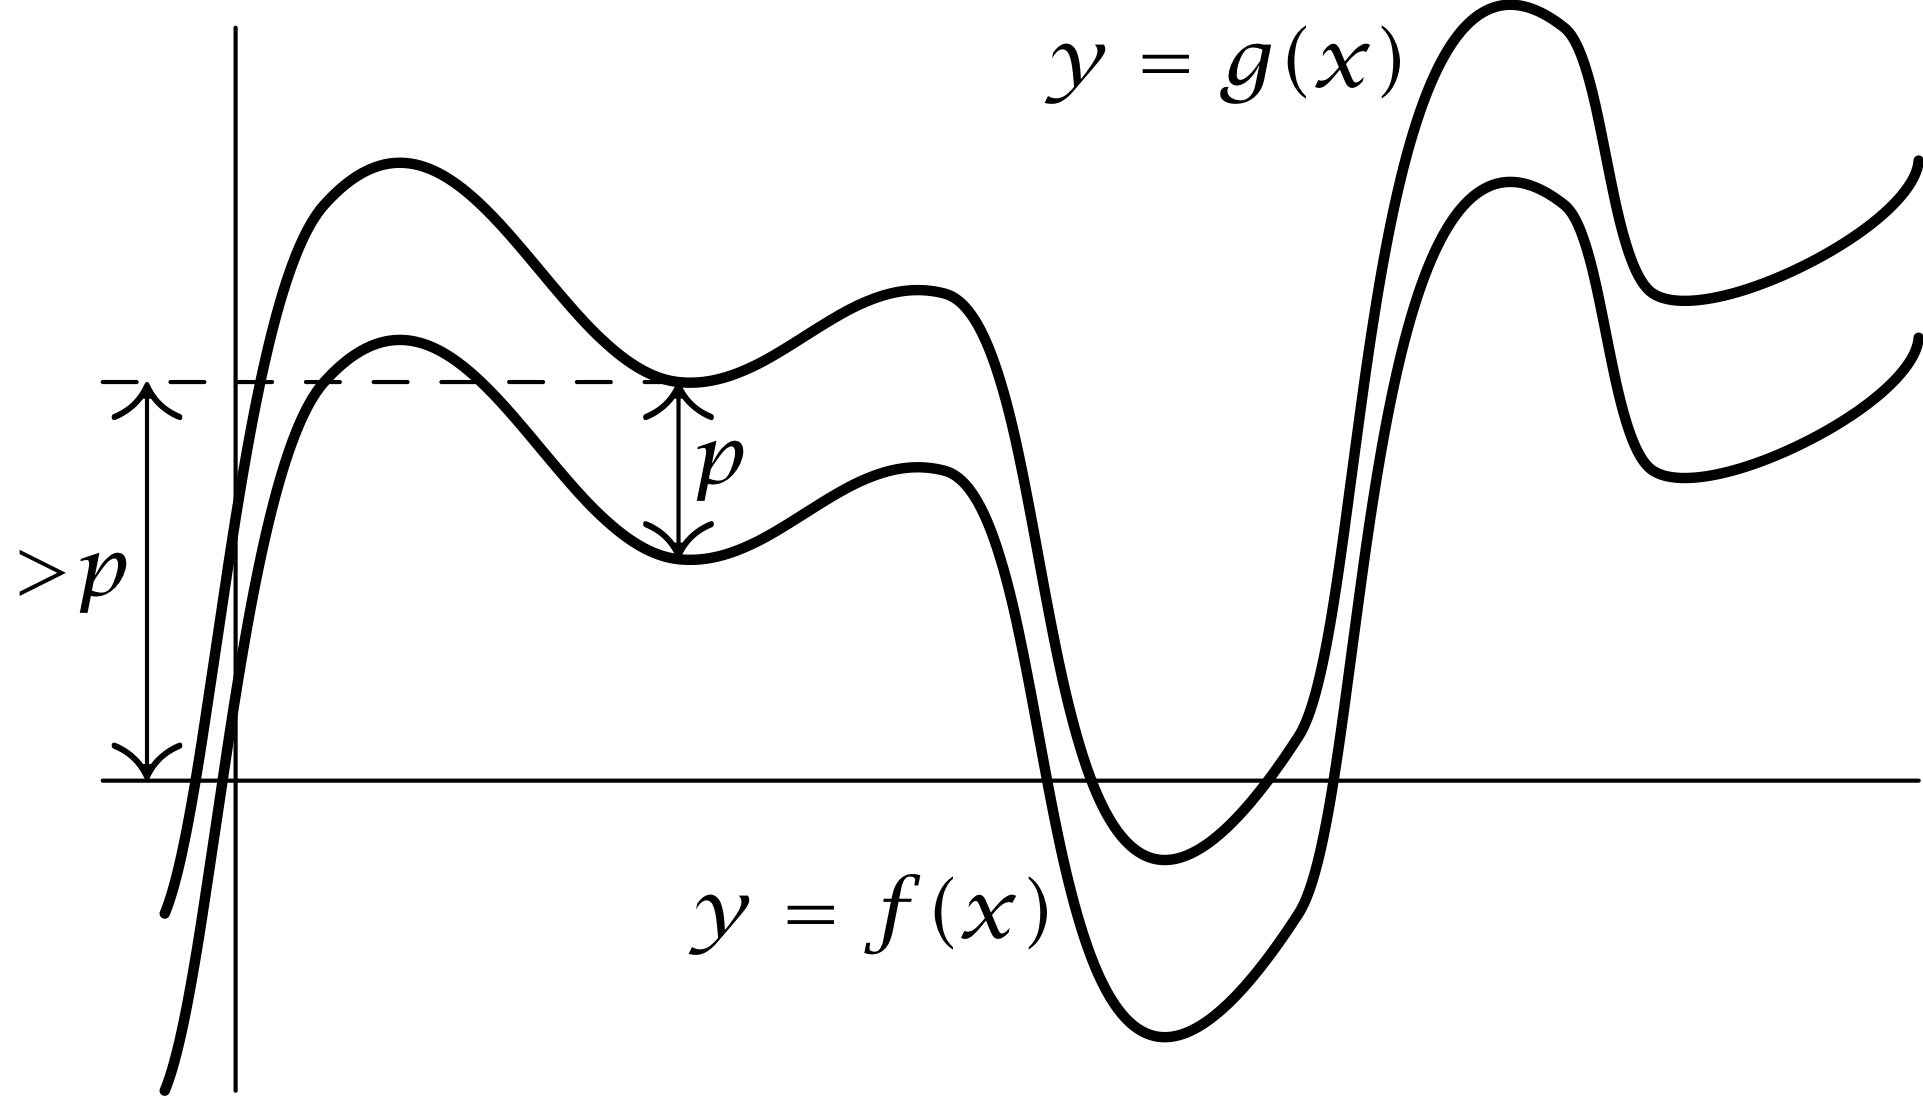
\includegraphics{PDF/samerealroots.jpg}}
%texpreamble
%("  \usepackage{amsmath}
% \usepackage[LY1]{fontenc}
% \usepackage[expert,LY1,mylucidascale]{mylucidabr}
% ");
%defaultpen(  fontcommand("\normalfont") + fontsize(10) ); 
%
%from graph access *;
%unitsize(0.75cm);
%
%pen thickpen = linewidth(1.25);
%
%
%path f = (0.1,-2){NNE}.. tension 2 ..(1,2)..(3,1)..(4.5,1.5) ..(6.5,-1).. tension 2 ..(8,3).. tension 2 ..(8.5,1.5)..tension 2 ..(10,2.25);
%
%draw(f, thickpen);
%draw( shift(0,1)*f, thickpen);
%
%label("$p$", (3,1.5) , 0.5*E);
%draw( (3,1)--(3,2), Arrows(TeXHead,2));
%
%draw( (-0.25,-0.25)--(10,-0.25) );
%draw( (0.5,-2)--(0.5,4) );
%
%draw( (-0.25,2)--(3,2), dashed);
%draw( (0,-0.25)--(0,2), Arrows(TeXHead,2));
%label("${>} p$", (0,.875), 0.5*W);
%
%label("$y = f(x)$", (4.1,-1) );
%label("$y = g(x)$", (6.1,3.8) );



\begin{exercises}

\item \label{CocpctSUSp}
 Use restriction of scalars to
construct cocompact arithmetic subgroups of  $\SU(m,n)$ and
$\Sp(m,n)$ for all $m$ and~$n$.
\hint{See the proof of \cref{SOmnHasCocpct}.}

\item \label{Isotypic->irredNotAbsSimpleEx}
The proof of \cref{Isotypic->irred} assumes that $G^i_\complex$ is simple for every~$i$. Remove this assumption.
\hint{You may use \cref{GxC=GxGiff} (without proof), and you will need the full strength of \cref{rReal+sImag}.}

\item \label{CpctFactorNotCocpct}
 Construct a noncocompact, irreducible lattice in $\SL(2,\real)
\times \SO(3)$.
 \hint{The free group $F_2$ is a noncocompact lattice in
$\SL(2,\real)$. Let $\Gamma$ be the graph of a homomorphism
$F_2 \to \SO(3)$ that has dense image.}

\item \label{NotCpct->UnipD}
In the proof of \cref{SO15xSO3H->Cocpct}, show there exists $v \in ( \quaternion^{a,b}_F )^3$, such that $\tau_r(v)^\transpose A v = 0$.
\hint{If $g$ is a nontrivial unipotent element of~$G_F$, then there is some $w$, such that $g$ fixes the nonzero vector $v = g w - w$.}

\item \label{rescalepoly}
 \begin{enumerate}
 \item Suppose $g(x)$ is a monic polynomial of degree~$n$,
and assume $k \in \integer \smallsetminus \{0\}$, such that $k \, g(x) \in
\integer[x]$. Show $k^n g(x/k) \in \integer[x]$.
 \item Suppose $g(x)$ is a monic, integral polynomial of
degree~$n$, and $p$~is a prime. Show that
 $p^{2n}g(x/p^2) \equiv x^n \pmod{p^2}$.
 \item Suppose $g(x)$ and $h(x)$ are monic polynomials, and
$k$~and~$n$ are nonzero integers, such that $h(x) =
k^ng(x/k)$. Show that
 $$\min \{\, |h(t)| \mid h'(t) = 0 \,\}
 = k^n \min \{\, |g(t)| \mid g'(t) = 0 \,\} .$$
 \end{enumerate}

 \end{exercises}














\begin{notes}

A proof of the classification of complex semisimple Lie algebras (\ref{AlmostAllOverC},\ref{EFGOverCRem}) can be found in standard texts, such as \cite[Thm.~11.4, pp.~57--58, and Thm.~18.4, p.~101]{Humphreys-LieAlg}.

The classification of real simple Lie algebras
(\cref{RformsComplete}) was
obtained by \'E.\,Cartan \cite{Cartan-RSimple}. (The
intervening decades have led to enormous simplifications in
the proof.) 

In \cref{GaloisCohoRealFormsSect,QFormsOfSLnSect}, our cohomological approach to the classification of $F$-forms of the classical groups is based on \cite[\S2.3]{PlatonovRapinchukBook}, where full details can be found. See \cite{Tits-Classification} for a list of all $F$-forms (mostly without proof), including exceptional groups (intended for readers familiar with root systems). The special case of real forms (including exceptional groups) is proved, by a somewhat different approach, in \cite[Chap.~10]{HelgasonBook}. 

\Cref{ArithLattsAreClassical} is due to Weil \cite{Weil-Classical}. 
A proof (together with
\cref{GxC=,GFxC}) is in \cite[\S2.3,
pp.~78--92]{PlatonovRapinchukBook}. We copied \pref{GxC=},
\pref{FClassicalDefn}, and~\pref{GFxC} from
\cite[p.~92]{PlatonovRapinchukBook}, except that
\cite{PlatonovRapinchukBook} uses a different description of
the groups in~\fullref{FClassicalDefn}{SUSO}
\csee{G=SU(skewHerm)}.

\Cref{AutMatInnerEx} is an easy special case of the \thmindex{Skolem-Noether}{Skolem-Noether Theorem}, which can be found in texts on ring theory, such as \cite[\S12.6, p.~230]{Pierce-AssocAlgs}.

\Cref{DivAlg/R}, the classification of division algebras over~$\real$, is due to Frobenius (1878), and a proof can be found in \cite[pp.~452--453]{Jacobson-BasicAlgebra1}. 

\Cref{BorelHarderLocGlob} is due to A.\,Borel and G.\,Harder \cite{BorelHarder-exist}.
See \cite{Johnson-isotypic} for an explicit construction of~$\widehat G$ in the special case where the simple factors of~$G$ are classical.

G.\,Prasad (personal communication) supplied \cref{SO15xSO3H->Cocpct}. It is a counterexample to the noncocompact part of \cite[Thm.~C]{Johnson-isotypic}, which erroneously states that isotypic groups with no compact factors have both cocompact and noncocompact irreducible lattices.

\Cref{GxC=GxGiff} is a consequence of \cite[Prop.~1 of App.~2, p.~385]{Bourbaki-LieGrpsLieAlgs2}, since a connected Lie group is simple if and only if its adjoint representation has no nonzero, proper, invariant subspaces. 

\thmindex{Meyer's}{Meyer's Theorem} (used in
the proof of \cref{QrankGap}) can be found in
\cite[Thm.~1 of \S1.7 and Thm.~5 of \S1.6, pp.~61
and~51]{BorevichShafarevich} or \cite[Cor.~2 of \S4.3.2,
p.~43]{Serre-CourseArith}.

\end{notes}



\begin{references}{99}

%\bibitem{Borel-IntroGrpArith}
%A.\,Borel:
%\emph{Introduction aux Groupes Arithm\'etiques}.
%%Publications de l'Institut de MathŽmatique de l'UniversitŽ de Strasbourg, XV. ActualitŽs Scientifiques et Industrielles, No. 1341 
%Hermann, Paris, 1969.
%ISBN 978-2705613419,
%\MR{0244260}, 

\bibitem{BorelHarder-exist}
 A.\,Borel and G.\,Harder:
 Existence of discrete cocompact subgroups of reductive
groups over local fields,
 \emph{J. Reine Angew. Math.} 298 (1978) 53--64.
 \MR{0483367},
 \maynewline
 \url{http://eudml.org/doc/151965}
% \url{http://www.digizeitschriften.de/dms/resolveppn/?PPN=GDZPPN00219452X}
 
\bibitem{BorevichShafarevich}
 Z.\,I.\,Borevich and I.\,R.\,Shafarevich:
 \emph{Number Theory,}
 Academic Press, New York, 1966.
\MR{0195803}

\bibitem{Bourbaki-LieGrpsLieAlgs2}
N.\,Bourbaki:
\emph{Lie Groups and Lie Algebras, Chapters 7--9}. 
%Translated from the 1975 and 1982 French originals by Andrew Pressley. Elements of Mathematics (Berlin). 
Springer, Berlin, 2005. 
ISBN 3-540-43405-4,
\MR{2109105}

\bibitem{Cartan-RSimple}
 \'E.\,Cartan:
 Les groupes r\'eels simples finis et continus,
 \emph{Ann. Sci. \'Ecole Norm. Sup.} 31 (1914) 263--355.
 \Zbl{45.1408.03},
 \maynewline
 \url{http://www.numdam.org/item?id=ASENS_1914_3_31__263_0}

%\bibitem{Chevalley-spinor}
% C.\,Chevalley:
% \emph{The Algebraic Theory of Spinors and Clifford
%Algebras,}
% Collected Works, Vol.~2, Springer, Berlin, 1997.
% \MR{1636473}

%\bibitem{Dieudonne-Geom}
% J.\,Dieudonn\'e:
% \emph{La G\'eom\'etrie des Groupes Classiques, 2nd ed.,}
% Springer, Berlin, 1963.
% \MR{0158011}

\bibitem{HelgasonBook} 
S.\,Helgason:
\emph{Differential Geometry, Lie Groups, and Symmetric Spaces.}
% Pure and Applied Mathematics, 80. 
Academic Press, New York, 1978.
ISBN 0-12-338460-5,
\MR{0514561}

\bibitem{Humphreys-LieAlg}
 J.\,E.\,Humphreys:
 \emph{Introduction to Lie Algebras and Representation
Theory.}
 Springer, {Berlin Heidelberg New York}, 1972.
 \MR{0323842}

\bibitem{Jacobson-BasicAlgebra1}
N.\,Jacobson:
\emph{Basic Algebra~I, 2nd~ed.}.
Freeman, New York, 1985. 
ISBN 0-7167-1480-9,
\MR{0780184}

\bibitem{Johnson-isotypic}
 F.\,E.\,A.\,Johnson:
 On the existence of irreducible discrete subgroups in
isotypic Lie groups of classical type,
 \emph{Proc. London Math. Soc.} (3) 56 (1988) 51--77.
 \MR{0915530},
 \maynewline
 \url{http://dx.doi.org/10.1112/plms/s3-56.1.51}

\bibitem{Pierce-AssocAlgs}
R.\,S.\,Pierce:
 \emph{Associative Algebras.}
 Springer, New York, 1982.
 ISBN 0-387-90693-2,
 \MR{0674652}

\bibitem{PlatonovRapinchukBook}
 V.\,Platonov and A.\,Rapinchuk: 
 \emph{Algebraic Groups and Number Theory.}
 Academic Press, Boston, 1994.
 ISBN 0-12-558180-7,
 \MR{1278263}
 
\bibitem{Serre-CourseArith}
 J.--P.\,Serre:
 \emph{A Course in Arithmetic,}
 Springer, New York 1973.
 \MR{0344216}

 \bibitem{Tits-Classification}
J.\,Tits:
Classification of algebraic semisimple groups,
in A.\,Borel and G.\,D.\,Mostow, eds.:
\emph{Algebraic Groups and Discontinuous Subgroups (Boulder, Colo., 1965)},
Amer. Math. Soc., Providence, R.I., 1966,  pp.~33--62.
\MR{0224710}

\bibitem{Weil-Classical}
 A.\,Weil:
 Algebras with involution and the classical groups,
 \emph{J. Indian Math. Soc.} 24 (1960) 589--623.
\MR{0136682} % no URL available @@@

 \end{references}
